% Options for packages loaded elsewhere
\PassOptionsToPackage{unicode}{hyperref}
\PassOptionsToPackage{hyphens}{url}
\PassOptionsToPackage{dvipsnames,svgnames,x11names}{xcolor}
%
\documentclass[
doublespace,
  times]{anzsauth}

\usepackage{amsmath,amssymb}
\usepackage{iftex}
\ifPDFTeX
  \usepackage[T1]{fontenc}
  \usepackage[utf8]{inputenc}
  \usepackage{textcomp} % provide euro and other symbols
\else % if luatex or xetex
  \usepackage{unicode-math}
  \defaultfontfeatures{Scale=MatchLowercase}
  \defaultfontfeatures[\rmfamily]{Ligatures=TeX,Scale=1}
\fi
\usepackage{lmodern}
\ifPDFTeX\else  
    % xetex/luatex font selection
\fi
% Use upquote if available, for straight quotes in verbatim environments
\IfFileExists{upquote.sty}{\usepackage{upquote}}{}
\IfFileExists{microtype.sty}{% use microtype if available
  \usepackage[]{microtype}
  \UseMicrotypeSet[protrusion]{basicmath} % disable protrusion for tt fonts
}{}
\makeatletter
\@ifundefined{KOMAClassName}{% if non-KOMA class
  \IfFileExists{parskip.sty}{%
    \usepackage{parskip}
  }{% else
    \setlength{\parindent}{0pt}
    \setlength{\parskip}{6pt plus 2pt minus 1pt}}
}{% if KOMA class
  \KOMAoptions{parskip=half}}
\makeatother
\usepackage{xcolor}
\setlength{\emergencystretch}{3em} % prevent overfull lines
\setcounter{secnumdepth}{5}
% Make \paragraph and \subparagraph free-standing
\makeatletter
\ifx\paragraph\undefined\else
  \let\oldparagraph\paragraph
  \renewcommand{\paragraph}{
    \@ifstar
      \xxxParagraphStar
      \xxxParagraphNoStar
  }
  \newcommand{\xxxParagraphStar}[1]{\oldparagraph*{#1}\mbox{}}
  \newcommand{\xxxParagraphNoStar}[1]{\oldparagraph{#1}\mbox{}}
\fi
\ifx\subparagraph\undefined\else
  \let\oldsubparagraph\subparagraph
  \renewcommand{\subparagraph}{
    \@ifstar
      \xxxSubParagraphStar
      \xxxSubParagraphNoStar
  }
  \newcommand{\xxxSubParagraphStar}[1]{\oldsubparagraph*{#1}\mbox{}}
  \newcommand{\xxxSubParagraphNoStar}[1]{\oldsubparagraph{#1}\mbox{}}
\fi
\makeatother

\usepackage{color}
\usepackage{fancyvrb}
\newcommand{\VerbBar}{|}
\newcommand{\VERB}{\Verb[commandchars=\\\{\}]}
\DefineVerbatimEnvironment{Highlighting}{Verbatim}{commandchars=\\\{\}}
% Add ',fontsize=\small' for more characters per line
\usepackage{framed}
\definecolor{shadecolor}{RGB}{241,243,245}
\newenvironment{Shaded}{\begin{snugshade}}{\end{snugshade}}
\newcommand{\AlertTok}[1]{\textcolor[rgb]{0.68,0.00,0.00}{#1}}
\newcommand{\AnnotationTok}[1]{\textcolor[rgb]{0.37,0.37,0.37}{#1}}
\newcommand{\AttributeTok}[1]{\textcolor[rgb]{0.40,0.45,0.13}{#1}}
\newcommand{\BaseNTok}[1]{\textcolor[rgb]{0.68,0.00,0.00}{#1}}
\newcommand{\BuiltInTok}[1]{\textcolor[rgb]{0.00,0.23,0.31}{#1}}
\newcommand{\CharTok}[1]{\textcolor[rgb]{0.13,0.47,0.30}{#1}}
\newcommand{\CommentTok}[1]{\textcolor[rgb]{0.37,0.37,0.37}{#1}}
\newcommand{\CommentVarTok}[1]{\textcolor[rgb]{0.37,0.37,0.37}{\textit{#1}}}
\newcommand{\ConstantTok}[1]{\textcolor[rgb]{0.56,0.35,0.01}{#1}}
\newcommand{\ControlFlowTok}[1]{\textcolor[rgb]{0.00,0.23,0.31}{\textbf{#1}}}
\newcommand{\DataTypeTok}[1]{\textcolor[rgb]{0.68,0.00,0.00}{#1}}
\newcommand{\DecValTok}[1]{\textcolor[rgb]{0.68,0.00,0.00}{#1}}
\newcommand{\DocumentationTok}[1]{\textcolor[rgb]{0.37,0.37,0.37}{\textit{#1}}}
\newcommand{\ErrorTok}[1]{\textcolor[rgb]{0.68,0.00,0.00}{#1}}
\newcommand{\ExtensionTok}[1]{\textcolor[rgb]{0.00,0.23,0.31}{#1}}
\newcommand{\FloatTok}[1]{\textcolor[rgb]{0.68,0.00,0.00}{#1}}
\newcommand{\FunctionTok}[1]{\textcolor[rgb]{0.28,0.35,0.67}{#1}}
\newcommand{\ImportTok}[1]{\textcolor[rgb]{0.00,0.46,0.62}{#1}}
\newcommand{\InformationTok}[1]{\textcolor[rgb]{0.37,0.37,0.37}{#1}}
\newcommand{\KeywordTok}[1]{\textcolor[rgb]{0.00,0.23,0.31}{\textbf{#1}}}
\newcommand{\NormalTok}[1]{\textcolor[rgb]{0.00,0.23,0.31}{#1}}
\newcommand{\OperatorTok}[1]{\textcolor[rgb]{0.37,0.37,0.37}{#1}}
\newcommand{\OtherTok}[1]{\textcolor[rgb]{0.00,0.23,0.31}{#1}}
\newcommand{\PreprocessorTok}[1]{\textcolor[rgb]{0.68,0.00,0.00}{#1}}
\newcommand{\RegionMarkerTok}[1]{\textcolor[rgb]{0.00,0.23,0.31}{#1}}
\newcommand{\SpecialCharTok}[1]{\textcolor[rgb]{0.37,0.37,0.37}{#1}}
\newcommand{\SpecialStringTok}[1]{\textcolor[rgb]{0.13,0.47,0.30}{#1}}
\newcommand{\StringTok}[1]{\textcolor[rgb]{0.13,0.47,0.30}{#1}}
\newcommand{\VariableTok}[1]{\textcolor[rgb]{0.07,0.07,0.07}{#1}}
\newcommand{\VerbatimStringTok}[1]{\textcolor[rgb]{0.13,0.47,0.30}{#1}}
\newcommand{\WarningTok}[1]{\textcolor[rgb]{0.37,0.37,0.37}{\textit{#1}}}

\providecommand{\tightlist}{%
  \setlength{\itemsep}{0pt}\setlength{\parskip}{0pt}}\usepackage{longtable,booktabs,array}
\usepackage{calc} % for calculating minipage widths
% Correct order of tables after \paragraph or \subparagraph
\usepackage{etoolbox}
\makeatletter
\patchcmd\longtable{\par}{\if@noskipsec\mbox{}\fi\par}{}{}
\makeatother
% Allow footnotes in longtable head/foot
\IfFileExists{footnotehyper.sty}{\usepackage{footnotehyper}}{\usepackage{footnote}}
\makesavenoteenv{longtable}
\usepackage{graphicx}
\makeatletter
\def\maxwidth{\ifdim\Gin@nat@width>\linewidth\linewidth\else\Gin@nat@width\fi}
\def\maxheight{\ifdim\Gin@nat@height>\textheight\textheight\else\Gin@nat@height\fi}
\makeatother
% Scale images if necessary, so that they will not overflow the page
% margins by default, and it is still possible to overwrite the defaults
% using explicit options in \includegraphics[width, height, ...]{}
\setkeys{Gin}{width=\maxwidth,height=\maxheight,keepaspectratio}
% Set default figure placement to htbp
\makeatletter
\def\fps@figure{htbp}
\makeatother

% The following \newcommands are intended for use in the *current*
% document ("protoType"). It is unlikely that authors of papers submitted
% to the Journal will need them.  (Of course if it turns out that you
% do indeed need them, then by all means feel free to make use of them.)
%%%%%%%%%%%%%%%%%%%%%%%%%%%%%%%%%%%%%%%%%%%%%%%%%%%%%%%%%%%%%%%%%%%%%%%%%%%%%%
\usepackage{lipsum}

\newcommand\BibTeX{{\rmfamily B\kern-.05em \textsc{i\kern-.025em b}\kern-.08em
T\kern-.1667em\lower.7ex\hbox{E}\kern-.125emX}}
\newcommand\MiKTeX{{\rmfamily M\kern-.05em \textsc{i\kern-.025em K}\kern-.08em
T\kern-.1667em\lower.7ex\hbox{E}\kern-.125emX}}
\newcommand\PracTeX{{\rmfamily P\kern-.05em \textsc{r\kern-.025em a\kern-.025em
c}\kern-.08em
T\kern-.1667em\lower.7ex\hbox{E}\kern-.125emX}}
%%%%%%%%%%%%%%%%%%%%%%%%%%%%%%%%%%%%%%%%%%%%%%%%%%%%%%%%%%%%%%%%%%%%%%%%%%%%%%

\usepackage{pmboxdraw}
\makeatletter
\@ifpackageloaded{caption}{}{\usepackage{caption}}
\AtBeginDocument{%
\ifdefined\contentsname
  \renewcommand*\contentsname{Table of contents}
\else
  \newcommand\contentsname{Table of contents}
\fi
\ifdefined\listfigurename
  \renewcommand*\listfigurename{List of Figures}
\else
  \newcommand\listfigurename{List of Figures}
\fi
\ifdefined\listtablename
  \renewcommand*\listtablename{List of Tables}
\else
  \newcommand\listtablename{List of Tables}
\fi
\ifdefined\figurename
  \renewcommand*\figurename{Figure}
\else
  \newcommand\figurename{Figure}
\fi
\ifdefined\tablename
  \renewcommand*\tablename{Table}
\else
  \newcommand\tablename{Table}
\fi
}
\@ifpackageloaded{float}{}{\usepackage{float}}
\floatstyle{ruled}
\@ifundefined{c@chapter}{\newfloat{codelisting}{h}{lop}}{\newfloat{codelisting}{h}{lop}[chapter]}
\floatname{codelisting}{Listing}
\newcommand*\listoflistings{\listof{codelisting}{List of Listings}}
\makeatother
\makeatletter
\makeatother
\makeatletter
\@ifpackageloaded{caption}{}{\usepackage{caption}}
\@ifpackageloaded{subcaption}{}{\usepackage{subcaption}}
\makeatother

\ifLuaTeX
  \usepackage{selnolig}  % disable illegal ligatures
\fi
\usepackage[]{natbib}
\bibliographystyle{anzsj}
\usepackage{bookmark}

\IfFileExists{xurl.sty}{\usepackage{xurl}}{} % add URL line breaks if available
\urlstyle{same} % disable monospaced font for URLs
\hypersetup{
  pdftitle={Software for Automated Residual Plot Assessment: autovi and autovi.web},
  pdfauthor={Weihao Li; Dianne Cook; Emi Tanaka; Susan VanderPlas; Klaus Ackermann},
  pdfkeywords={statistical software, statistical graphics, data
visualization, visual inference, computer vision, machine
learning, hypothesis testing, reression analysis},
  colorlinks=true,
  linkcolor={blue},
  filecolor={Maroon},
  citecolor={Blue},
  urlcolor={Blue},
  pdfcreator={LaTeX via pandoc}}

\usepackage{moreverb}
\usepackage{url}
\usepackage{grffile}
\usepackage[UKenglish]{isodate}

%%%%%%%%%%%%%%%%%%%%%%%%%%%%%%%%%%%%%%%%%%%%%%%%%%%%%%%%%%%%%%%%%%%%%%%%%%%%%%

% The year in the following may need to be updated!
\def\volumeyear{2024}

% The following command ("obviously") effects line numbering
% of the document.

\usepackage{lineno}
\linenumbers


\def\firstletters{\bgroup \catcode`-=10 \catcode`(=10 \filA}
\def\filA#1{\filB#1 {\end} }
\def\filB#1#2 {\ifx\end#1\egroup \else#1 \expandafter\filB\fi}

\runningheads{
Software for Automated Residual Plot Assessment
}{
\firstletters{WEIHAO}LI, \firstletters{DIANNE}COOK, \firstletters{EMI}TANAKA, \firstletters{SUSAN}VANDERPLAS, AND  \firstletters{KLAUS}ACKERMANN
}

\title{Software for Automated Residual Plot Assessment: autovi and
autovi.web}
\usepackage{etoolbox}
\makeatletter
\providecommand{\subtitle}[1]{% add subtitle to \maketitle
  \apptocmd{\@title}{\par {\large #1 \par}}{}{}
}
\makeatother
\subtitle{ANZJS Quarto Template}

\author{
Weihao Li\addressnum{1},
Dianne Cook\addressnum{1},
Emi Tanaka\addressnum{2},
Susan VanderPlas\addressnum{3} and
Klaus Ackermann
\addressnum{1}
}
\affiliation{
Monash University,
The Australian National University and
University of Nebraska
}

\address{
\addressnum{1} Department of Econometrics and Business
Statistics, Monash University, Wellington Road, VIC 3800, Australia\\
\addressnum{2} Biological Data Science Institute, The Australian
National University, 46 Sullivan's Creek Road, ACT 2600, Australia\\
\addressnum{3} Department of Statistics, University of Nebraska, Hardin
Hall, 3310 Holdrege St Suite 340, Lincoln, NE 68583, United States\\
\hspace*{1ex} Email: \texttt{weihao.li@monash.edu}    
}


\date{2024}
\begin{document}

\begin{abstract}
Regression software is widely available today, but tools for effective
diagnostics are still lagging. Perhaps, one of the reasons is that it is
hard. Conventional tests, that would make the task easy, are often too
sensitive, which would result in adequate models being abandoned if the
analyst strictly adhered to the test decision. The recommended advice is
to have the analyst assess the strength of patterns in residual plots.
This requires human effort and also suffers from the potential for
inconsistent decisions from different analysts. Using a lineup protocol
can help to alleviate inconsistency, but requires even more human
effort. This is the type of task where a robot might be employed to do
the disagreeable work that currently requires a human. Here we describe
a new R package that includes a computer vision model for automated
assessment of residual plots, and an accompanying Shiny app for ease of
use. For a user-provided sample of residuals, it predicts a measure of
visual signal strength (VSS) and provides a suite of supporting
information to assist the analyst diagnose their model fit.
\end{abstract}

\keywords{statistical software; statistical graphics; data
visualization; visual inference; computer vision; machine
learning; hypothesis testing; reression analysis}
          
\ack{The author acknowledges that this template is based on the latex
template for Australian and New Zealand Journal of Statistics and
intersperses some text from the original prototype document.
\newline\vspace{1ex}\newline Opinions and attitudes expressed in this
document, which are not explicitly designated as Journal policy, are
those of the author and are \emph{not} necessarily endorsed by the
Journal, its editorial board, its publisher Wiley or by the Australian
Statistical Publishing Association Inc.}

\maketitle


\section{Introduction}\label{sec-autovi-introduction}

Regression analysis is a fundamental statistical technique widely used
for modeling data from many fields. To diagnose the fit of a model it is
recommended that the residuals are plotted. If the fit is good, any
variation remaining should be noise, consistent with sampling from a
distribution specified by the error model. Deviations that might be
observed from a residual plot are non-normality, heteroscedasticity, and
other associations with the fitted values. In \citet{li2024plot}, we
demonstrated that visual methods for assessing residuals are
advantageous over conventional tests due to their reduced sensitivity to
minor departures. Building on this, \citet{li2024automated} introduced a
computer vision model aimed at alleviating the human effort required for
visual assessment of residual plots. The next step is to deliver the use
of the computer vision model to potential users, so that it can be
widely used to the benefit of the analytics community.

Software for regression analysis tools is widely available. The
Comprehensive R Archive Network (CRAN) \citep{hornik2012comprehensive}
hosts a vast array of packages, many of which provide tools to diagnose
models using residual plots. These packages can be broadly categorized
into three groups: general-purpose, enhanced visual diagnostics, and
visual diagnostics with statistical testing.

General-purpose regression analysis tools are the most widely used group
of packages. While not specifically designed for graphical diagnostics
of residuals in linear regression, they include this functionality as
part of a broader suite of statistical tools. For example, the
\texttt{stats} package \citep{stats} offers standard diagnostic plots
such as residuals vs.~fitted values, quantile-quantile (Q-Q) plots, and
residuals vs.~leverage plots. Additional packages like \texttt{jtools}
\citep{jtools}, \texttt{olsrr} \citep{olsrr}, \texttt{rockchalk}
\citep{rockchalk}, and \texttt{ggResidpanel} \citep{ggresidpanel}
provide similar graphical diagnostics, often with alternative aesthetics
or interactive features. All of these tools deliver the types of
diagnostic plots outlined in the classical text by
\citet{cook1982residuals}. However, as discussed in \citet{li2024plot},
relying solely on subjective assessments of these plots can lead to
issues, such as over-interpreting random patterns as model violations.

The second group consists of enhanced visual diagnostics tools, which
provide advanced aids for interpreting diagnostic plots. For instance,
\texttt{ecostats} \citep{warton_global_2023} incorporates simulation
envelopes into residual plots, while \texttt{DHARMa} \citep{dharma}
compares empirical quantiles (0.25, 0.5, and 0.75) of scaled residuals
to their theoretical counterparts. \texttt{DHARMa} is particularly
focused on detecting model violations such as heteroscedasticity,
incorrect functional forms, and issues specific to generalized linear
and mixed-effect models, like over/under-dispersion. It also includes
annotations from conventional tests, displayed as labels or text within
the plot, to help avoid misinterpretation.

The third group, visual diagnostics with statistical testing, offers
tools for formally testing patterns observed in diagnostic plots
\citep{buja2009statistical}. A common method for visual testing of
residual plots is the lineup protocol, where the true residual plot is
embedded within a set of null plots generated by simulating residuals
under the null hypothesis \(H_0\) that the regression model is correctly
specified. Observers are asked to identify the plot that appears most
different from the others. If a significant proportion of observers
correctly identify the true residual plot, it provides evidence against
\(H_0\), as the true residual plot should be indistinguishable from the
null plots if all residuals are generated by the same process, according
to \citet{buja2009statistical}. Packages in this group, such as
\texttt{nullabor} \citep{nullabor}, \texttt{HLMdiag}
\citep{loy2014hlmdiag}, and \texttt{regressinator}
\citep{regressinator}, enable users to compare observed residual plots
with samples from null distributions, helping to quantify the
significance of any detected patterns.

However, as discussed in \citet{li2024automated}, the lineup protocol
has significant limitations in large-scale applications due dependence
on human labor. Thus a computer vision model was developed with an
associated statistical testing procedure to automate the assessment of
residual plots. This model takes a residual plot and a vector of
auxiliary variables (such as the number of observations) as inputs and
outputs the predicted visual signal strength (VSS). This strength
estimates the distance between the residual distribution of the fitted
regression model and the reference distribution assumed under correct
model specification.

To make the statistical testing procedure and trained computer vision
model widely accessible, we developed the R package \texttt{autovi}, and
a web interface, \texttt{autovi.web} to make it easy for users to
automatically read their residual plots with the trained computer vision
model.

The remainder of this paper is structured as follows:
Section~\ref{sec-autovi} provides a detailed documentation of the
\texttt{autovi} package, including its usage and infrastructure.
Section~\ref{sec-autovi-web} focuses on the \texttt{autovi.web}
interface, describing its design and usage, along with illustrative
examples. Finally, Section~\ref{sec-autovi-conclusion} presents the main
conclusions of this work.

\section{R package: autovi}\label{sec-autovi}

The main purpose of \texttt{autovi} is to provide rejection decisions
and \(p\)-values for testing whether a regression model is correctly
specified. The package introduces a novel approach to automating
statistical analysis, particularly in the interpretation of residual
plots. The name \texttt{autovi} stands for automated visual inference.
While initially designed for linear regression residual diagnostics, it
has the potential to be extended to broader visual inference
applications, as we discuss in section
Section~\ref{sec-autovi-infrastructure}.

\subsection{Implementation}\label{sec-autovi-implementation}

The \texttt{autovi} package is built on the \texttt{bandicoot}
object-oriented programming (OOP) system \citep{bandicoot}, marking a
departure from R's traditional S3 generic system. This OOP architecture
enhances flexibility and modularity, allowing users to redefine key
functions through method overriding. While similar functionality could
be achieved using R's S3 system with generic functions, the OOP
framework offers a more structured and extensible foundation for the
package.

The \texttt{autovi} infrastructure effectively integrates multiple
programming languages and libraries into a comprehensive analytical
tool. It relies on five core libraries from Python and R, each playing a
critical role in the analysis pipeline. In Python, \texttt{pillow}
\citep{clark2015pillow} handles image processing tasks such as reading
and resizing PNG files of residual plots, then converting them into
input tensors for further analysis. The \texttt{TensorFlow}
\citep{abadi2016tensorflow} library, a key component of modern machine
learning, is used to predict the VSS of these plots through a
pre-trained convolutional neural network.

In the R environment, \texttt{autovi} utilizes several libraries.
\texttt{ggplot2} \citep{ggplot2} generates the initial residual plots,
saved as PNG files for visual input. The \texttt{cassowaryr}
\citep{mason2022cassowaryr} library computes scagnostics (scatter plot
diagnostics), providing numerical features that capture statistical
properties of the plots. These scagnostics complement the visual
analysis by offering quantitative metrics as secondary input to the
computer vision model. The \texttt{reticulate} \citep{reticulate}
package bridges R and Python, enabling seamless communication between
the two languages and supporting the integrated infrastructure.

\subsection{Installation}\label{installation}

The \texttt{autovi} package is available on CRAN. It is actively
developed and maintained, with the latest updates accessible on GitHub
at \url{https://github.com/TengMCing/autovi}. The code discussed in this
paper is based on \texttt{autovi} version 0.4.1.

The package includes internal functions to check the current Python
environment used by the \texttt{reticulate} package. If the necessary
Python packages are not installed in the Python interpreter, an error
will be raised. If you want to select a specific Python environment, you
can do so by calling the \texttt{reticulate::use\_python()} function
before using the \texttt{autovi} package.

\subsection{Usage}\label{sec-autovi-usage}

To get started quickly, only three function calls are needed to obtain a
summary of the automated residual assessment:

\begin{Shaded}
\begin{Highlighting}[]
\FunctionTok{library}\NormalTok{(autovi) }
\NormalTok{checker }\OtherTok{\textless{}{-}} \FunctionTok{residual\_checker}\NormalTok{(}\FunctionTok{lm}\NormalTok{(dist }\SpecialCharTok{\textasciitilde{}}\NormalTok{ speed, }\AttributeTok{data =}\NormalTok{ cars))}
\NormalTok{checker}\SpecialCharTok{$}\FunctionTok{check}\NormalTok{() }
\end{Highlighting}
\end{Shaded}

\begin{verbatim}
\end{verbatim}

\begin{verbatim}
-- <AUTO_VI object>
Status:
 - Fitted model: lm
 - Keras model: UNKNOWN
    - Output node index: 1
 - Result:
    - Observed visual signal strength: 3.162 (p-value = 0.0396)
    - Null visual signal strength: [100 draws]
       - Mean: 1.274
       - Quantiles: 
          ╔═════════════════════════════════════════════════╗
          ║   25%    50%    75%    80%    90%    95%    99% ║
          ║0.8021 1.1109 1.5751 1.6656 1.9199 2.6564 3.3491 ║
          ╚═════════════════════════════════════════════════╝
    - Bootstrapped visual signal strength: [100 draws]
       - Mean: 2.786 (p-value = 0.05941)
       - Quantiles: 
          ╔══════════════════════════════════════════╗
          ║  25%   50%   75%   80%   90%   95%   99% ║
          ║2.452 2.925 3.173 3.285 3.463 3.505 3.652 ║
          ╚══════════════════════════════════════════╝
    - Likelihood ratio: 0.7275 (boot) / 0.06298 (null) = 11.55 
\end{verbatim}

The three functions are explained as follows:

\begin{enumerate}
\def\labelenumi{\arabic{enumi}.}
\tightlist
\item
  Load the \texttt{autovi} package using the \texttt{library()}
  function.
\item
  Create a checker object with a linear regression model.
\item
  Call the \texttt{check()} method of the checker, which, by default,
  predicts the VSS for the true residual plot, 100 null plots, and 100
  bootstrapped plots, storing the predictions internally. A concise
  report of the check results is then printed.
\end{enumerate}

The summary reports key findings such as the VSS of the true residual
plot and the \(p\)-value of the automated visual test. The \(p\)-value
is the ratio of null plots that have VSS greater than or equal to that
of the true residual plot. We typically reject the null hypothesis when
the \(p\)-value is smaller than or equal to a desired significance
level, such as 5\%. The report also provides sample quantiles of VSS for
null and bootstrapped plots, helping to explain the severity and
likelihood of model violations.

Although the \(p\)-value is sufficient for automated decision-making,
users can visually inspect the original residual plot alongside a sample
null plot. This visual comparison can clarify why \(H_0\) is either
rejected or not, and help identify potential remedies. The
\texttt{plot\_pair()} and \texttt{plot\_lineup()} methods facilitate
this comparison.

\begin{Shaded}
\begin{Highlighting}[]
\NormalTok{checker}\SpecialCharTok{$}\FunctionTok{plot\_pair}\NormalTok{()}
\end{Highlighting}
\end{Shaded}

\begin{figure}[H]

\centering{

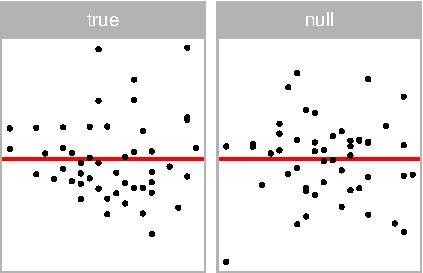
\includegraphics[width=1\textwidth,height=\textheight]{autovi_paper_files/figure-pdf/fig-plot-pair-1.pdf}

}

\caption{\label{fig-plot-pair}True plot alongside one null plot, for
quick comparison.}

\end{figure}%

The \texttt{plot\_pair()} method (Figure~\ref{fig-plot-pair}) displays
the true residual plot on the left and a single null plot on the right.
If a full lineup was shown, the true residual plot would be embedded in
a page of null plots. Users should look for any distinct visual patterns
in the true residual plot that are absent in the null plot. Running
these functions multiple times can help any visual suspicions, as each
execution generates new random null plots for comparison.

The package offers a straightforward visualization of the assessment
result through the \texttt{summary\_plot()} function.

\begin{Shaded}
\begin{Highlighting}[]
\NormalTok{checker}\SpecialCharTok{$}\FunctionTok{summary\_plot}\NormalTok{()}
\end{Highlighting}
\end{Shaded}

\begin{figure}[H]

\centering{

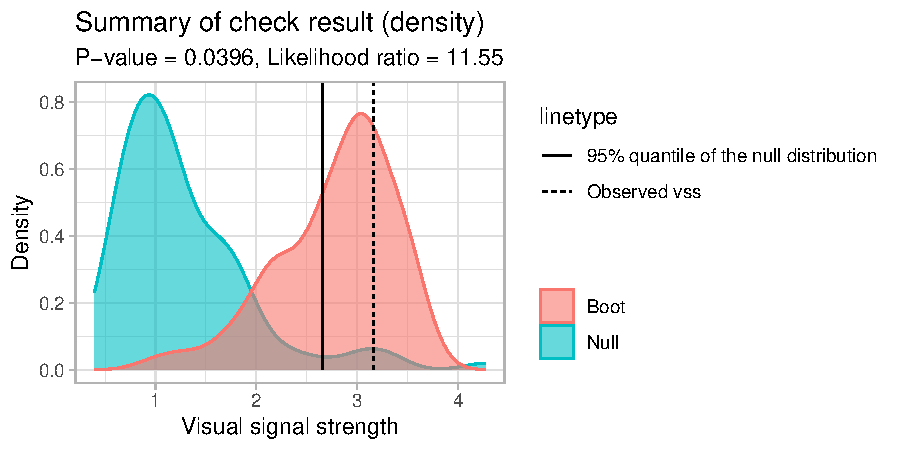
\includegraphics[width=1\textwidth,height=\textheight]{autovi_paper_files/figure-pdf/fig-summary-plot-1.pdf}

}

\caption{\label{fig-summary-plot}Summary plot comparing the densities of
VSS for bootstrapped residual samples (red) relative to VSS for null
plots (blue).}

\end{figure}%

In the result, shown in Figure~\ref{fig-summary-plot}, the blue area
represents the density of VSS for null residual plots, while the red
area shows the density for bootstrapped residual plots. The dashed line
indicates the VSS of the true residual plot, and the solid line marks
the critical value at a 95\% significance level. The \(p\)-value and the
likelihood ratio are displayed in the subtitle. The likelihood ratio
represents the ratio of the likelihood of observing the VSS of the true
residual plot from the bootstrapped distribution compared to the null
distribution.

Interpreting the plot involves several key aspects. If the dashed line
falls to the right of the solid line, it suggests rejecting the null
hypothesis. The degree of overlap between the red and blue areas
indicates similarity between the true residual plot and null plots;
greater overlap suggests more similarity. Lastly, the portion of the red
area to the right of the solid line represents the percentage of
bootstrapped models considered to have model violations.

This visual summary provides an intuitive way to assess the model's fit
and potential violations, allowing users to quickly grasp the results of
the automated analysis.

\subsection{Modularized Infrastructure}\label{sec-autovi-infrastructure}

\begin{figure}

\centering{

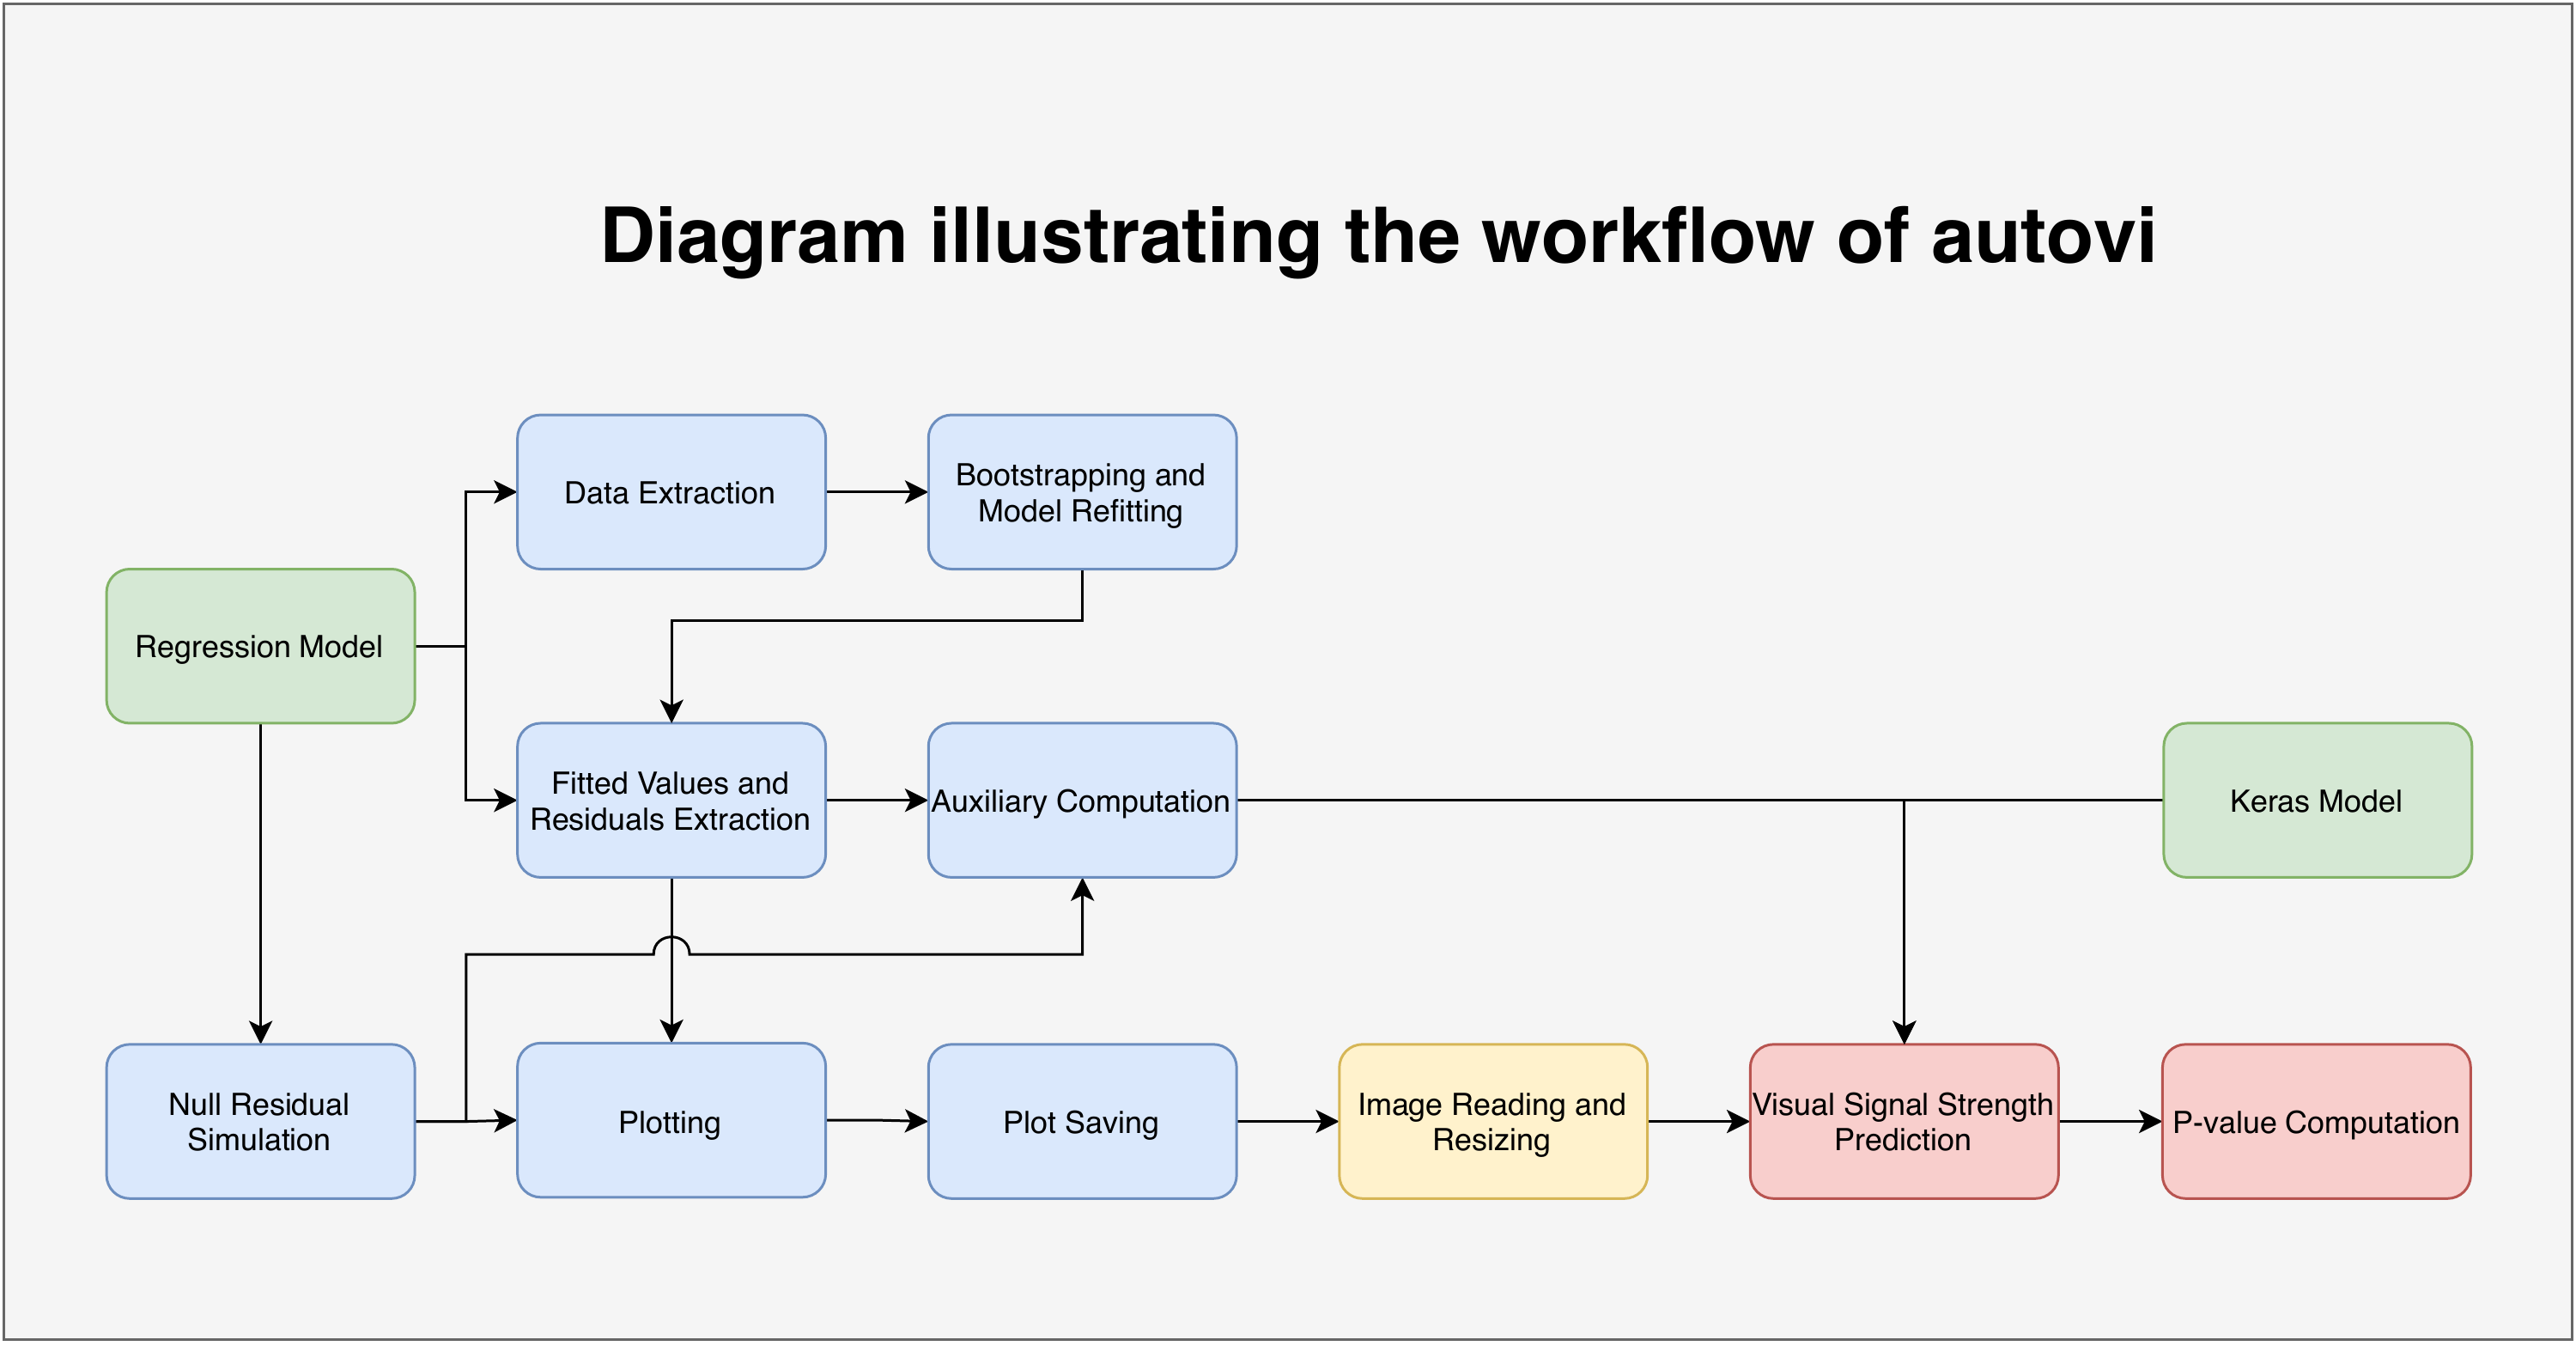
\includegraphics[width=1\textwidth,height=\textheight]{autovi_paper_files/figure-pdf/fig-autovi-diag-1.png}

}

\caption{\label{fig-autovi-diag}Diagram illustrating the infrastructure
of the R package autovi. The modules in green are primary inputs
provided by users. Modules in blue are overridable methods that can be
modified to accommodate users' specific needs. The module in yellow is a
pre-defined non-overridable method. The modules in red are primary
outputs of the package.}

\end{figure}%

The initial motivation for developing \texttt{autovi} was to create a
convenient interface for sharing the models described and trained in
\citet{li2024automated}. However, recognizing that the classical normal
linear regression model represents a restricted class of models, we
sought to avoid limiting the potential for future extensions, whether by
the original developers or other users. As a result, the package was
designed to function seamlessly with linear regression models with
minimal modification and few required arguments, while also
accommodating other classes of models through partial infrastructure
substitution. This modular and customizable design allows
\texttt{autovi} to handle a wide range of residual diagnostics tasks.

The infrastructure of \texttt{autovi} consists of ten core modules: data
extraction, bootstrapping and model refitting, fitted values and
residuals extraction, auxiliary computation, null residual simulation,
plotting, plot saving, image reading and resizing, VSS prediction, and
\(p\)-value computation. Each module is designed with minimal dependency
on the preceding modules, allowing users to customize parts of the
infrastructure without affecting its overall integrity. An overview of
this infrastructure is illustrated in Figure~\ref{fig-autovi-diag}.

The modules for VSS prediction and \(p\)-value computation are
predefined and cannot be overridden, although users can interact with
them directly through function arguments. Similarly, the image reading
and resizing module is fixed but will adapt to different Keras models by
checking their input shapes. The remaining seven modules are designed to
be overridable, enabling users to tailor the infrastructure to their
specific needs. These modules are discussed in detail in the following
sections.

\subsubsection{Initialization}\label{initialization}

An \texttt{autovi} checker can be initialized by supplying two primary
inputs, including a regression model object, such as an \texttt{lm}
object representing the result of a linear regression model, and a
trained computer vision model compatible with the \texttt{Keras}
\citep{chollet2015keras} Application Programming Interface (API), to the
\texttt{AUTO\_VI} class constructor \texttt{auto\_vi()}. The
\texttt{residual\_checker()} introduced in
Section~\ref{sec-autovi-usage} is a thin wrapper around
\texttt{auto\_vi()}, which will call \texttt{get\_keras\_model()} during
initialization. \texttt{get\_keras\_model()} is a function to download a
trained computer vision model (described in \citet{li2024automated})
from GitHub. ``vss\_phn\_32'' specifies a model that predicts VSS and is
trained on residuals with polynomial, heteroskedasticity, and
non-normality patterns (phn). More details about the hosted models will
be provided in Section~\ref{sec-trained-model-hosting}.

The input of the constructor will be stored as attributes of the checker
and can be accessed by the user through the \texttt{\$} operator.

\begin{Shaded}
\begin{Highlighting}[]
\FunctionTok{library}\NormalTok{(autovi)}
\NormalTok{checker }\OtherTok{\textless{}{-}} \FunctionTok{auto\_vi}\NormalTok{(}\AttributeTok{fitted\_model =} \FunctionTok{lm}\NormalTok{(dist }\SpecialCharTok{\textasciitilde{}}\NormalTok{ speed, }\AttributeTok{data =}\NormalTok{ cars), }
                   \AttributeTok{keras\_model =} \FunctionTok{get\_keras\_model}\NormalTok{(}\StringTok{"vss\_phn\_32"}\NormalTok{))}
\end{Highlighting}
\end{Shaded}

Optionally, the user may specify the node index of the output layer of
the trained computer vision model to be monitored by the checker via the
\texttt{node\_index} argument if there are multiple output nodes. This
is particularly useful for multiclass classifiers when the user wants to
use one of the nodes as a VSS indicator.

After initializing the object, you can print the checker to view its
status.

\begin{Shaded}
\begin{Highlighting}[]
\NormalTok{── }\SpecialCharTok{\textless{}}\NormalTok{AUTO\_VI object}\SpecialCharTok{\textgreater{}}
\NormalTok{Status}\SpecialCharTok{:}
 \SpecialCharTok{{-}}\NormalTok{ Fitted model}\SpecialCharTok{:}\NormalTok{ lm}
 \SpecialCharTok{{-}}\NormalTok{ Keras model}\SpecialCharTok{:}\NormalTok{ (None, }\DecValTok{32}\NormalTok{, }\DecValTok{32}\NormalTok{, }\DecValTok{3}\NormalTok{) }\SpecialCharTok{+}\NormalTok{ (None, }\DecValTok{5}\NormalTok{) }\OtherTok{{-}\textgreater{}}\NormalTok{ (None, }\DecValTok{1}\NormalTok{)}
    \SpecialCharTok{{-}}\NormalTok{ Output node index}\SpecialCharTok{:} \DecValTok{1}
 \SpecialCharTok{{-}}\NormalTok{ Result}\SpecialCharTok{:}\NormalTok{ UNKNOWN }
\end{Highlighting}
\end{Shaded}

The status includes the list of regression model classes (as provided by
the built-in \texttt{class()} function), the input and output shapes of
the Keras model in the standard \texttt{Numpy} format
\citep{harris2020array}, the output node index being monitored, and the
assessment result. If no check has been run yet, the assessment result
will display as ``UNKNOWN''.

\subsubsection{Fitted Values and Residuals
Extraction}\label{fitted-values-and-residuals-extraction}

To be able to predict VSS for a residual plot, both fitted values and
residuals are needed to be extracted from the regression model object
supplied by the user. In R, statistical models like \texttt{lm} (linear
model) and \texttt{glm} (generalized linear model) typically support the
use of generic functions such as \texttt{fitted()} and \texttt{resid()}
to retrieve these values. The \texttt{get\_fitted\_and\_resid()} method,
called by the checker, relies on these generic functions by default.
However, generic functions only work with classes that have appropriate
method implementations. Some regression modeling packages may not fully
adhere to the \texttt{stats} package guidelines for implementing these
functions. In such cases, overriding the method becomes necessary.

By design, the \texttt{get\_fitted\_and\_resid()} method accepts a
regression model object as input and returns a \texttt{tibble} (a modern
presentation of the \texttt{data.frame}) with two columns:
\texttt{.fitted} and \texttt{.resid}, representing the fitted values and
residuals, respectively. If no input is supplied, the method uses the
regression model object stored in the checker. Although modules in the
\texttt{autovi} infrastructure make minimal assumptions about other
modules, they do require strictly defined input and output formats to
ensure data validation and prevent fatal bugs. Therefore, any overridden
method should follow to these conventions.

\begin{Shaded}
\begin{Highlighting}[]
\NormalTok{checker}\SpecialCharTok{$}\FunctionTok{get\_fitted\_and\_resid}\NormalTok{()}
\end{Highlighting}
\end{Shaded}

\begin{verbatim}
# A tibble: 50 x 2
   .fitted .resid
     <dbl>  <dbl>
 1   -1.85   3.85
 2   -1.85  11.8 
 3    9.95  -5.95
 4    9.95  12.1 
 5   13.9    2.12
 6   17.8   -7.81
 7   21.7   -3.74
 8   21.7    4.26
 9   21.7   12.3 
10   25.7   -8.68
# i 40 more rows
\end{verbatim}

\subsubsection{Data Extraction}\label{data-extraction}

For linear regression model in R, the model frame contains all the data
required by a formula for evaluation. This is essential for
bootstrapping and refitting the model when constructing a bootstrapped
distribution of VSS. Typically, the model frame can be extracted from
the regression model object using the \texttt{model.frame()} generic
function, which is the default method used by \texttt{get\_data()}.
However, some regression models do not use a formula or are evaluated
differently, potentially lacking a model frame. In such cases, users can
either provide the data used to fit the regression model through the
\texttt{data} argument when constructing the checker, or customize the
method to better suit their needs. It's worth noting that this module is
only necessary if bootstrapping is required, as the model frame is not
used in other modules of the infrastructure.

The \texttt{get\_data()} method accepts a regression model object as
input and returns a \texttt{data.frame} representing the model frame of
the fitted regression model. If no input is supplied, the regression
model stored in the checker will be used.

\begin{Shaded}
\begin{Highlighting}[]
\NormalTok{checker}\SpecialCharTok{$}\FunctionTok{get\_data}\NormalTok{() }\SpecialCharTok{|\textgreater{}} 
  \FunctionTok{head}\NormalTok{()}
\end{Highlighting}
\end{Shaded}

\begin{verbatim}
  dist speed
1    2     4
2   10     4
3    4     7
4   22     7
5   16     8
6   10     9
\end{verbatim}

\subsubsection{Bootstrapping and Model
Refitting}\label{bootstrapping-and-model-refitting}

Bootstrapping a regression model typically involves sampling the
observations with replacement and refitting the model with the
bootstrapped data. The \texttt{boot\_method()} method follows this
bootstrapping scheme by default. It accepts a fitted regression model
and a \texttt{data.frame} as inputs, and returns a \texttt{tibble} of
bootstrapped residuals. If no inputs are provided, the method uses the
regression model stored in the checker and the result of the
\texttt{get\_data()} method.

Note that instead of calling \texttt{get\_data()} implicitly within the
method, it is used as part of the default argument definition. This
approach allows users to bypass the \texttt{get\_data()} method entirely
and directly supply a \texttt{data.frame} to initiate the bootstrap
process. Many other methods in \texttt{autovi} adopt this principle when
possible, where dependencies are explicitly listed in the formal
arguments. This design choice enhances the reusability and isolation of
modules, offers better control for testing, and simplifies the overall
process.

\begin{Shaded}
\begin{Highlighting}[]
\NormalTok{checker}\SpecialCharTok{$}\FunctionTok{boot\_method}\NormalTok{(}\AttributeTok{data =}\NormalTok{ checker}\SpecialCharTok{$}\FunctionTok{get\_data}\NormalTok{())}
\end{Highlighting}
\end{Shaded}

\begin{verbatim}
# A tibble: 50 x 2
   .fitted .resid
     <dbl>  <dbl>
 1   27.0   -2.96
 2   38.8  -12.8 
 3   34.8   -8.82
 4   27.0  -13.0 
 5   11.2    4.76
 6   42.7   -2.68
 7   42.7   -2.68
 8   38.8  -18.8 
 9   38.8   15.2 
10   -4.47   6.47
# i 40 more rows
\end{verbatim}

\subsubsection{Auxiliary Computation}\label{auxiliary-computation}

As described in \citet{li2024automated}, in some cases, a residual plot
alone may not provide enough information to accurately determine VSS.
For instance, when the points in the residual plot have significant
overlap, the trend and shape of the residual pattern can be difficult to
discern. Including auxiliary variables, such as the number of
observations, as additional inputs to the computer vision model can be
beneficial. To address this, \texttt{autovi} includes internal functions
within the checker that automatically detect the number of inputs
required by the provided Keras model. If multiple inputs are necessary,
the checker invokes the \texttt{auxiliary()} method to compute these
additional inputs.

The \texttt{auxiliary()} method takes a \texttt{data.frame} containing
fitted values and residuals as input and returns a \texttt{data.frame}
with five numeric columns. These columns represent four scagnostics ---
``Monotonic'', ``Sparse'', ``Striped'', and ``Splines'' --- calculated
using the \texttt{cassowaryr} package, as well as the number of
observations. This approach is consistent with the training process of
the computer vision models described in \citet{li2024automated}. If no
\texttt{data.frame} is provided, the method will default to retrieving
fitted values and residuals by calling
\texttt{get\_fitted\_and\_resid()}.

Technically, any Keras-implemented computer vision model can be adapted
to accept an image as the primary input and additional variables as
secondary inputs by adding a data pre-processing layer before the actual
input layer. If users wish to override \texttt{auxiliary()}, the output
should be a \texttt{data.frame} with a single row and the number of
columns such that its concatenation matches the number of parameters for
the corresponding layer in the supplied Keras model.

\begin{Shaded}
\begin{Highlighting}[]
\NormalTok{checker}\SpecialCharTok{$}\FunctionTok{auxiliary}\NormalTok{()}
\end{Highlighting}
\end{Shaded}

\begin{verbatim}
# A tibble: 1 x 5
  measure_monotonic measure_sparse measure_splines measure_striped     n
              <dbl>          <dbl>           <dbl>           <dbl> <int>
1            0.0621          0.470          0.0901            0.62    50
\end{verbatim}

\subsubsection{Null Residual Simulation}\label{sec-autovi-null-method}

A fundamental element of the automated residual assessment described in
\citet{li2024automated} is comparing the VSS of null plots with that of
the true residual plot. However, due to the variety of regression
models, there is no universal method for simulating null residuals that
are consistent with model assumptions. Fortunately, for classical normal
linear regression models, null residuals can be effectively simulated
using the residual rotation method, as outlined in
\citet{buja2009statistical}. This process involves generating random
draws from a standard normal distribution, regressing these draws on the
original predictors, and then rescaling the resulting residuals by the
ratio of the residual sum of squares to the that of the original linear
regression model. Other regression models, such as \texttt{glm}
(generalized linear model) and \texttt{gam} (generalized additive
model), generally cannot use this method to efficiently simulate null
residuals. Therefore, it is recommended that users override the
\texttt{null\_method()} to suit their specific model. The
\texttt{null\_method()} takes a fitted regression model as input,
defaulting to the regression model stored in the checker, and returns a
\texttt{tibble}.

\begin{Shaded}
\begin{Highlighting}[]
\NormalTok{checker}\SpecialCharTok{$}\FunctionTok{null\_method}\NormalTok{()}
\end{Highlighting}
\end{Shaded}

\begin{verbatim}
# A tibble: 50 x 2
   .fitted  .resid
     <dbl>   <dbl>
 1   -1.85  18.2  
 2   -1.85  -0.765
 3    9.95 -12.8  
 4    9.95  18.6  
 5   13.9    2.57 
 6   17.8    7.03 
 7   21.7  -11.1  
 8   21.7  -13.2  
 9   21.7  -12.6  
10   25.7    3.57 
# i 40 more rows
\end{verbatim}

\subsubsection{Plotting}\label{plotting}

Plotting is a crucial aspect of residual plot diagnostics because
aesthetic elements like marker size, marker color, and auxiliary lines
impact the presentation of information. There are computer vision models
trained to handle images captured in various scenarios. For example, the
VGG16 model \citep{simonyan2014very} can classify objects in images
taken under different lighting conditions and is robust to image
rotation. However, data plots are a special type of image as the
plotting style can always be consistent if controlled properly.
Therefore, we assume computer vision models built for reading residual
plots will be trained with residual plots of a specific aesthetic style.
In this case, it is best to predict plots using the same style for
optimal performance. The plotting method \texttt{plot\_resid()} handles
this aspect.

\texttt{plot\_resid()} accepts a \texttt{data.frame} containing fitted
values and residuals, along with several customization options: a
\texttt{ggplot} theme, an \texttt{alpha} value to control the
transparency of data points, a \texttt{size} value to set the size of
data points, and a \texttt{stroke} value to define the thickness of data
point edges. Additionally, it includes four Boolean arguments to toggle
the display of axes, legends, grid lines, and a horizontal red line. By
default, it replicates the style we used to generate the training
samples for the computer vision models described in
\citet{li2024automated}. In brief, the residual plot omits axis text and
ticks, titles, and background grid lines, featuring only a red line at
\(y = 0\). It retains only the necessary components of a residual plot.
If the computer vision model is trained with a different but consistent
aesthetic style, \texttt{plot\_resid()} should be overridden.

The method returns a \texttt{ggplot} object
(Figure~\ref{fig-autovi-plot-resid}), which can be saved as a PNG file
in the following module. If no data is provided, the method will use
\texttt{get\_fitted\_and\_resid()} to retrieve the fitted values and
residuals from the regression model stored in the checker.

\begin{Shaded}
\begin{Highlighting}[]
\NormalTok{checker}\SpecialCharTok{$}\FunctionTok{plot\_resid}\NormalTok{()}
\end{Highlighting}
\end{Shaded}

\begin{figure}[H]

\centering{

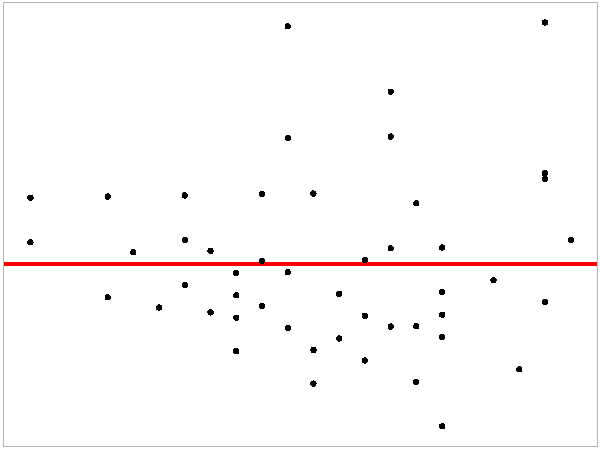
\includegraphics[width=1\textwidth,height=\textheight]{autovi_paper_files/figure-pdf/fig-autovi-plot-resid-1.pdf}

}

\caption{\label{fig-autovi-plot-resid}Residual plot of the regression
model stored in the checker.}

\end{figure}%

To manually generate true residual plots, null plots, or bootstrapped
residual plots, you can pass the corresponding \texttt{data.frame}
produced by the \texttt{get\_fitted\_and\_resid()},
\texttt{null\_method()}, and \texttt{boot\_method()} methods to the
\texttt{plot\_resid()} method, respectively.

\subsubsection{Plot Saving}\label{plot-saving}

Another key aspect of a standardized residual plot is its resolution. In
\citet{li2024automated}, we used an image format of 420 pixels in height
and 525 pixels in width. This resolution was chosen because the original
set, consisting of 20 residual plots arranged in a four by five grid,
was represented by an image of 2100 by 2100 pixels. The
\texttt{save\_plot()} method accepts a \texttt{ggplot} object as input
and saves it as a PNG file to the location specified by the
\texttt{path} argument. If no path is provided, the PNG file is saved to
a temporary file.

\begin{Shaded}
\begin{Highlighting}[]
\NormalTok{checker}\SpecialCharTok{$}\FunctionTok{plot\_resid}\NormalTok{() }\SpecialCharTok{|\textgreater{}} 
\NormalTok{  checker}\SpecialCharTok{$}\FunctionTok{save\_plot}\NormalTok{()}
\end{Highlighting}
\end{Shaded}

\begin{verbatim}
[1] "/var/folders/61/bv7_1qzs20x6fjb2rsv7513r0000gn/T//RtmpfYtMdO/file37817b7b5b6.png"
\end{verbatim}

\subsubsection{Image Reading and
Resizing}\label{image-reading-and-resizing}

When training computer vision models, it is common to test various input
sizes for the same architecture to identify the optimal setup. This
involves preparing the original training image at a higher resolution
than required and then resizing it to match the input size during
training. The \texttt{autovi} package includes a class,
\texttt{KERAS\_WRAPPER}, to simplify this process. This Keras wrapper
class features a method called \texttt{image\_to\_array()}, which reads
an image as a \texttt{PIL} image using the \texttt{pillow} Python
package, resizes it to the target input size required by the Keras
model, and converts it to a \texttt{Numpy} array.

To construct a \texttt{KERAS\_WRAPPER} object, you need to provide the
Keras model as the main argument. However, users generally do not need
to interact with this class directly, as the \texttt{autovi} checker
automatically invokes its methods when performing VSS predictions. The
\texttt{image\_to\_array()} method takes the path to the image file, the
target height, and the target width as inputs and returns a
\texttt{Numpy} array. If not specified, the target height and target
width will be retrieved from the input layer of the Keras model by the
\texttt{get\_input\_height()} and \texttt{get\_input\_width()} method of
\texttt{KERAS\_WRAPPER}.

The following code example demonstrate the way to manually generate the
true residual plot, save it as PNG file, and load it back as
\texttt{Numpy} array.

\begin{Shaded}
\begin{Highlighting}[]
\NormalTok{wrapper }\OtherTok{\textless{}{-}} \FunctionTok{keras\_wrapper}\NormalTok{(}\AttributeTok{keras\_model =}\NormalTok{ checker}\SpecialCharTok{$}\NormalTok{keras\_model)  }
\NormalTok{input\_array }\OtherTok{\textless{}{-}}\NormalTok{ checker}\SpecialCharTok{$}\FunctionTok{plot\_resid}\NormalTok{() }\SpecialCharTok{|\textgreater{}} 
\NormalTok{  checker}\SpecialCharTok{$}\FunctionTok{save\_plot}\NormalTok{() }\SpecialCharTok{|\textgreater{}}
\NormalTok{  wrapper}\SpecialCharTok{$}\FunctionTok{image\_to\_array}\NormalTok{()}
\NormalTok{input\_array}\SpecialCharTok{$}\NormalTok{shape}
\end{Highlighting}
\end{Shaded}

\begin{verbatim}
(1, 32, 32, 3)
\end{verbatim}

\subsubsection{Visual Signal Strength (VSS)
Prediction}\label{visual-signal-strength-vss-prediction}

VSS, as discussed in \citet{li2024automated}, estimates the distance
between the input residual plot and a theoretically good residual plot.
It can be defined in various ways, much like different methods for
measuring the distance between two points. This will not impact the
\texttt{autovi} infrastructure as long as the provided Keras model can
predict the intended measure.

There are several ways to obtain VSS from the checker, with the most
direct being the \texttt{vss()} method. By default, this method predicts
the VSS for the true residual plot. If a \texttt{ggplot} or a
\texttt{data.frame}, such as null residuals generated by the
\texttt{null\_method()}, is explicitly provided, the method will use
that input to predict VSS accordingly. Note that if a \texttt{ggplot} is
provided, auxiliary inputs must be supplied manually via the
\texttt{auxiliary} argument, as we assume that auxiliary variables can
not be computed directly from a \texttt{ggplot}.

Another way to obtain VSS is by calling the \texttt{check()} method.
This comprehensive method perform extensive diagnostics on the true
residual plot and store the VSS in the \texttt{check\_result} field of
the checker. Additionally, for obtaining VSS for null residual plots and
bootstrapped residual plots, there are two specialized methods,
\texttt{null\_vss()} and \texttt{boot\_vss()}, designed for this purpose
respectively.

Calling the \texttt{vss()} method without arguments will predict the VSS
for the true residual plot and return the result as a single-element
\texttt{tibble}.

\begin{Shaded}
\begin{Highlighting}[]
\NormalTok{checker}\SpecialCharTok{$}\FunctionTok{vss}\NormalTok{()}
\end{Highlighting}
\end{Shaded}

\begin{verbatim}
# A tibble: 1 x 1
    vss
  <dbl>
1  3.16
\end{verbatim}

Providing a \texttt{data.frame} of null residuals or a null residual
plot yields the same VSS.

\begin{Shaded}
\begin{Highlighting}[]
\NormalTok{null\_resid }\OtherTok{\textless{}{-}}\NormalTok{ checker}\SpecialCharTok{$}\FunctionTok{null\_method}\NormalTok{()}
\NormalTok{checker}\SpecialCharTok{$}\FunctionTok{vss}\NormalTok{(null\_resid)}
\end{Highlighting}
\end{Shaded}

\begin{verbatim}
# A tibble: 1 x 1
    vss
  <dbl>
1  1.23
\end{verbatim}

\begin{Shaded}
\begin{Highlighting}[]
\NormalTok{null\_resid }\SpecialCharTok{|\textgreater{}}
\NormalTok{  checker}\SpecialCharTok{$}\FunctionTok{plot\_resid}\NormalTok{() }\SpecialCharTok{|\textgreater{}}
\NormalTok{  checker}\SpecialCharTok{$}\FunctionTok{vss}\NormalTok{()}
\end{Highlighting}
\end{Shaded}

\begin{verbatim}
# A tibble: 1 x 1
    vss
  <dbl>
1  1.23
\end{verbatim}

The \texttt{null\_vss()} helper method primarily takes the number of
null plots as input. If the user wants to use a ad hoc null simulation
scheme, it can be provided via the \texttt{null\_method} argument.
Intermediate results, including null residuals and null plots, can be
returned by enabling \texttt{keep\_null\_data} and
\texttt{keep\_null\_plot}. The VSS, along with null residuals and null
plots, will be stored in a \texttt{tibble} with three columns. The
following code example demonstrates how to predict the VSS for five null
residual plots while keeping the intermediate results.

\begin{Shaded}
\begin{Highlighting}[]
\NormalTok{checker}\SpecialCharTok{$}\FunctionTok{null\_vss}\NormalTok{(}\DecValTok{5}\NormalTok{L, }
                 \AttributeTok{keep\_null\_data =} \ConstantTok{TRUE}\NormalTok{, }
                 \AttributeTok{keep\_null\_plot =} \ConstantTok{TRUE}\NormalTok{)}
\end{Highlighting}
\end{Shaded}

\begin{verbatim}
# A tibble: 5 x 3
    vss data              plot  
  <dbl> <list>            <list>
1 0.982 <tibble [50 x 2]> <gg>  
2 1.58  <tibble [50 x 2]> <gg>  
3 2.09  <tibble [50 x 2]> <gg>  
4 0.742 <tibble [50 x 2]> <gg>  
5 2.21  <tibble [50 x 2]> <gg>  
\end{verbatim}

The \texttt{boot\_vss()} helper method is similar to
\texttt{null\_vss()}, with some differences in argument names. The
following code example demonstrates how to predict the VSS for five
bootstrapped residual plots while keeping the intermediate results.

\begin{Shaded}
\begin{Highlighting}[]
\NormalTok{checker}\SpecialCharTok{$}\FunctionTok{boot\_vss}\NormalTok{(}\DecValTok{5}\NormalTok{L,}
                 \AttributeTok{keep\_boot\_data =} \ConstantTok{TRUE}\NormalTok{,}
                 \AttributeTok{keep\_boot\_plot =} \ConstantTok{TRUE}\NormalTok{)}
\end{Highlighting}
\end{Shaded}

\begin{verbatim}
# A tibble: 5 x 3
    vss data              plot  
  <dbl> <list>            <list>
1  3.12 <tibble [50 x 2]> <gg>  
2  2.37 <tibble [50 x 2]> <gg>  
3  2.87 <tibble [50 x 2]> <gg>  
4  1.85 <tibble [50 x 2]> <gg>  
5  3.66 <tibble [50 x 2]> <gg>  
\end{verbatim}

\subsubsection{\texorpdfstring{\(p\)-value
Computation}{p-value Computation}}\label{p-value-computation}

Once we have obtained the VSS from both the true residual plot and the
null plots, we can compute the \(p\)-value. This \(p\)-value represents
the ratio of plots with VSS greater than or equal to that of the true
residual plot. We can perform this calculation using the
\texttt{check()} method. The main inputs for this method are the number
of null plots and the number of bootstrapped plots to generate. If you
need to access intermediate residuals and plots, you can enable the
\texttt{keep\_data} and \texttt{keep\_plot} options. The method stores
the final result in the \texttt{check\_result} field of the object. To
obtain the p-value using the \texttt{check()} method, you can use the
following code.

\begin{Shaded}
\begin{Highlighting}[]
\NormalTok{checker}\SpecialCharTok{$}\FunctionTok{check}\NormalTok{(}\AttributeTok{boot\_draws =} \DecValTok{100}\NormalTok{L, }\AttributeTok{null\_draws =} \DecValTok{100}\NormalTok{L)}
\NormalTok{checker}\SpecialCharTok{$}\NormalTok{check\_result}\SpecialCharTok{$}\NormalTok{p\_value}
\end{Highlighting}
\end{Shaded}

\begin{verbatim}
[1] 0.02970297
\end{verbatim}

\subsection{Summary Plots}\label{summary-plots}

After executing the \texttt{check()} method, \texttt{autovi} offers two
visualization options for the assessment result through the
\texttt{summary\_plot()} method, including the density plot and the rank
plot. We have already discussed and interpreted the density plot in
Section~\ref{sec-autovi-usage}. Here, we would like to highlight the
flexibility in choosing which elements to display in the density plot as
shown in Figure~\ref{fig-autovi-summary-plot-option}. For instance, you
can omit the bootstrapped distribution by setting \texttt{boot\_dist} to
\texttt{NULL}. Similarly, you can hide the null distribution
(\texttt{null\_dist}), the \(p\)-value (\texttt{p\_value}), or the
likelihood ratio (\texttt{likelihood\_ratio}) as needed. The following
example demonstrates how to create a summary plot without the results
from bootstrapped plots.

\begin{Shaded}
\begin{Highlighting}[]
\NormalTok{checker}\SpecialCharTok{$}\FunctionTok{summary\_plot}\NormalTok{(}\AttributeTok{boot\_dist =} \ConstantTok{NULL}\NormalTok{,}
                     \AttributeTok{likelihood\_ratio =} \ConstantTok{NULL}\NormalTok{)}
\end{Highlighting}
\end{Shaded}

\begin{figure}[H]

\centering{

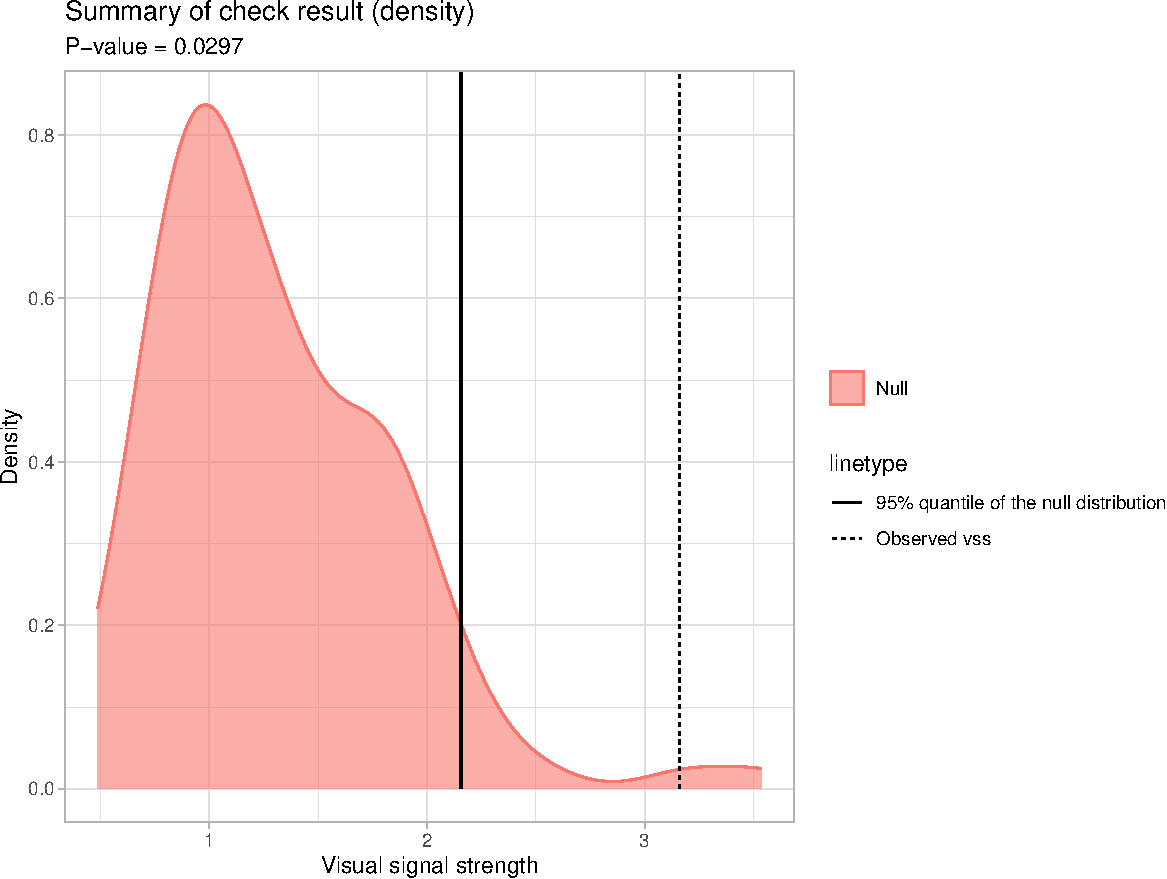
\includegraphics[width=1\textwidth,height=\textheight]{autovi_paper_files/figure-pdf/fig-autovi-summary-plot-option-1.pdf}

}

\caption{\label{fig-autovi-summary-plot-option}Density plot of the VSS
for null plots.}

\end{figure}%

This customization allows you to focus on specific aspects of the
assessment, tailoring the visualization to your analytical needs.

The rank plot (Figure~\ref{fig-autovi-rank-plot}), creating by setting
\texttt{type} to ``rank'', is a bar plot where the \(x\)-axis represents
the rank and the \(y\)-axis shows the VSS. The bar that is coloured in
red corresponding to the VSS of the true residual plot. By examining the
rank plot, you can intuitively understand how the observed VSS compares
to the null VSSs and identify any outliers in the null distribution.

\begin{Shaded}
\begin{Highlighting}[]
\NormalTok{checker}\SpecialCharTok{$}\FunctionTok{summary\_plot}\NormalTok{(}\AttributeTok{type =} \StringTok{"rank"}\NormalTok{)}
\end{Highlighting}
\end{Shaded}

\begin{figure}[H]

\centering{

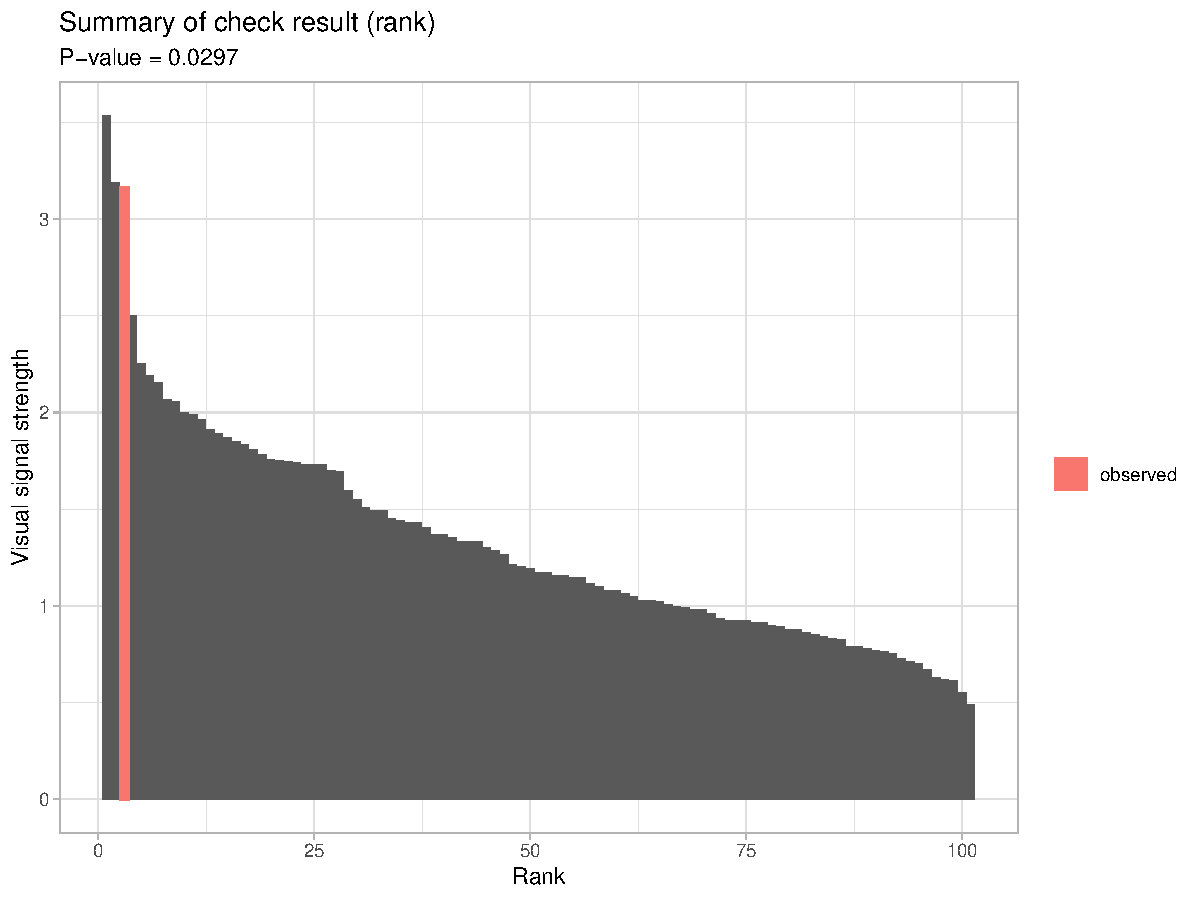
\includegraphics[width=1\textwidth,height=\textheight]{autovi_paper_files/figure-pdf/fig-autovi-rank-plot-1.pdf}

}

\caption{\label{fig-autovi-rank-plot}Rank plot of the VSS for null
plots.}

\end{figure}%

\subsection{Feature Extraction}\label{feature-extraction}

In addition to predicting VSS and computing \(p\)-values,
\texttt{autovi} offers methods to extract features from any layer of the
Keras model. To see which layers are available in the current Keras
model, you can use the \texttt{list\_layer\_name()} method from the
\texttt{KERAS\_WRAPPER} class.

The following code example lists the layer names of the currently used
Keras model:

\begin{Shaded}
\begin{Highlighting}[]
\NormalTok{wrapper }\OtherTok{\textless{}{-}} \FunctionTok{keras\_wrapper}\NormalTok{(checker}\SpecialCharTok{$}\NormalTok{keras\_model)}
\NormalTok{wrapper}\SpecialCharTok{$}\FunctionTok{list\_layer\_name}\NormalTok{()}
\end{Highlighting}
\end{Shaded}

\begin{verbatim}
 [1] "input_1"                  "tf.__operators__.getitem"
 [3] "tf.nn.bias_add"           "grey_scale"              
 [5] "block1_conv1"             "batch_normalization"     
 [7] "activation"               "block1_conv2"            
 [9] "batch_normalization_1"    "activation_1"            
[11] "block1_pool"              "dropout"                 
[13] "block2_conv1"             "batch_normalization_2"   
[15] "activation_2"             "block2_conv2"            
[17] "batch_normalization_3"    "activation_3"            
[19] "block2_pool"              "dropout_1"               
[21] "block3_conv1"             "batch_normalization_4"   
[23] "activation_4"             "block3_conv2"            
[25] "batch_normalization_5"    "activation_5"            
[27] "block3_conv3"             "batch_normalization_6"   
[29] "activation_6"             "block3_pool"             
[31] "dropout_2"                "block4_conv1"            
[33] "batch_normalization_7"    "activation_7"            
[35] "block4_conv2"             "batch_normalization_8"   
[37] "activation_8"             "block4_conv3"            
[39] "batch_normalization_9"    "activation_9"            
[41] "block4_pool"              "dropout_3"               
[43] "block5_conv1"             "batch_normalization_10"  
[45] "activation_10"            "block5_conv2"            
[47] "batch_normalization_11"   "activation_11"           
[49] "block5_conv3"             "batch_normalization_12"  
[51] "activation_12"            "block5_pool"             
[53] "dropout_4"                "global_max_pooling2d"    
[55] "additional_input"         "concatenate"             
[57] "dense"                    "dropout_5"               
[59] "activation_13"            "dense_1"                 
\end{verbatim}

Among these layers, the ``global\_max\_pooling2d'' layer is a 2D global
max pooling layer that outputs the results from the last convolutional
blocks. As \citet{simonyan2014very} noted, all preceding convolutional
blocks can be viewed as a large feature extractor. Consequently, the
output from this layer provides features that can be utilized for
various purposes, such as performing transfer learning.

To obtain the features, provide the layer name using the
\texttt{extract\_feature\_from\_layer} argument in the
\texttt{predict()} method. This will return a \texttt{tibble} with the
VSS and all features extracted from that layer. Each row corresponds to
one plot. The features will be flattened into 2D and named with the
prefix ``f\_'' followed by a number from one to the total number of
features.

\begin{Shaded}
\begin{Highlighting}[]
\NormalTok{checker}\SpecialCharTok{$}\FunctionTok{plot\_resid}\NormalTok{() }\SpecialCharTok{|\textgreater{}}
\NormalTok{  checker}\SpecialCharTok{$}\FunctionTok{save\_plot}\NormalTok{() }\SpecialCharTok{|\textgreater{}}
\NormalTok{  wrapper}\SpecialCharTok{$}\FunctionTok{image\_to\_array}\NormalTok{() }\SpecialCharTok{|\textgreater{}}
\NormalTok{  wrapper}\SpecialCharTok{$}\FunctionTok{predict}\NormalTok{(}\AttributeTok{auxiliary =}\NormalTok{ checker}\SpecialCharTok{$}\FunctionTok{auxiliary}\NormalTok{(),}
                  \AttributeTok{extract\_feature\_from\_layer =} \StringTok{"global\_max\_pooling2d"}\NormalTok{)}
\end{Highlighting}
\end{Shaded}

\begin{verbatim}
# A tibble: 1 x 257
    vss   f_1   f_2   f_3   f_4   f_5    f_6   f_7    f_8   f_9   f_10  f_11
  <dbl> <dbl> <dbl> <dbl> <dbl> <dbl>  <dbl> <dbl>  <dbl> <dbl>  <dbl> <dbl>
1  3.16 0.151     0     0     0     0 0.0203 0.109 0.0203     0 0.0834     0
# i 245 more variables: f_12 <dbl>, f_13 <dbl>, f_14 <dbl>, f_15 <dbl>,
#   f_16 <dbl>, f_17 <dbl>, f_18 <dbl>, f_19 <dbl>, f_20 <dbl>, f_21 <dbl>,
#   f_22 <dbl>, f_23 <dbl>, f_24 <dbl>, f_25 <dbl>, f_26 <dbl>, f_27 <dbl>,
#   f_28 <dbl>, f_29 <dbl>, f_30 <dbl>, f_31 <dbl>, f_32 <dbl>, f_33 <dbl>,
#   f_34 <dbl>, f_35 <dbl>, f_36 <dbl>, f_37 <dbl>, f_38 <dbl>, f_39 <dbl>,
#   f_40 <dbl>, f_41 <dbl>, f_42 <dbl>, f_43 <dbl>, f_44 <dbl>, f_45 <dbl>,
#   f_46 <dbl>, f_47 <dbl>, f_48 <dbl>, f_49 <dbl>, f_50 <dbl>, f_51 <dbl>, ...
\end{verbatim}

Alternatively, the \texttt{AUTO\_VI} class provides a way to extract
features using the \texttt{vss()} method. This method is essentially a
high-level wrapper around the \texttt{predict()} method of
\texttt{KERAS\_WRAPPER}, but it offers a more straightforward interface
and better default arguments.

The results from the previous code example can be replicated with a
single line of code as shown below.

\begin{Shaded}
\begin{Highlighting}[]
\NormalTok{checker}\SpecialCharTok{$}\FunctionTok{vss}\NormalTok{(}\AttributeTok{extract\_feature\_from\_layer =} \StringTok{"global\_max\_pooling2d"}\NormalTok{)}
\end{Highlighting}
\end{Shaded}

\begin{verbatim}
# A tibble: 1 x 257
    vss   f_1   f_2   f_3   f_4   f_5    f_6   f_7    f_8   f_9   f_10  f_11
  <dbl> <dbl> <dbl> <dbl> <dbl> <dbl>  <dbl> <dbl>  <dbl> <dbl>  <dbl> <dbl>
1  3.16 0.151     0     0     0     0 0.0203 0.109 0.0203     0 0.0834     0
# i 245 more variables: f_12 <dbl>, f_13 <dbl>, f_14 <dbl>, f_15 <dbl>,
#   f_16 <dbl>, f_17 <dbl>, f_18 <dbl>, f_19 <dbl>, f_20 <dbl>, f_21 <dbl>,
#   f_22 <dbl>, f_23 <dbl>, f_24 <dbl>, f_25 <dbl>, f_26 <dbl>, f_27 <dbl>,
#   f_28 <dbl>, f_29 <dbl>, f_30 <dbl>, f_31 <dbl>, f_32 <dbl>, f_33 <dbl>,
#   f_34 <dbl>, f_35 <dbl>, f_36 <dbl>, f_37 <dbl>, f_38 <dbl>, f_39 <dbl>,
#   f_40 <dbl>, f_41 <dbl>, f_42 <dbl>, f_43 <dbl>, f_44 <dbl>, f_45 <dbl>,
#   f_46 <dbl>, f_47 <dbl>, f_48 <dbl>, f_49 <dbl>, f_50 <dbl>, f_51 <dbl>, ...
\end{verbatim}

The argument \texttt{extract\_feature\_from\_layer} is also available in
other functions that build on the \texttt{vss()} method, including
\texttt{null\_vss()}, \texttt{boot\_vss()}, and \texttt{check()}.

\subsection{Trained Model Hosting}\label{sec-trained-model-hosting}

The trained computer vision models described in \citet{li2024automated}
are hosted on a GitHub repository at
\url{https://github.com/TengMCing/autovi_data}. Currently, there are six
models available. You can view them by calling
\texttt{list\_keras\_model()}, which will return a \texttt{tibble}
showing the input shape and a description of each model.

\begin{Shaded}
\begin{Highlighting}[]
\FunctionTok{list\_keras\_model}\NormalTok{() }\SpecialCharTok{|\textgreater{}}
  \FunctionTok{str}\NormalTok{()}
\end{Highlighting}
\end{Shaded}

\begin{verbatim}
tibble [6 x 11] (S3: tbl_df/tbl/data.frame)
 $ model_name          : chr [1:6] "vss_32" "vss_64" "vss_128" "vss_phn_32" ...
 $ path                : chr [1:6] "keras_model/vss_32.keras.zip" "keras_model/vss_64.keras.zip" "keras_model/vss_128.keras.zip" "keras_model/vss_phn_32.keras.zip" ...
 $ volume_path         : chr [1:6] "keras_model_volumes/vss_32.zip.001" "keras_model_volumes/vss_64.zip.001" "keras_model_volumes/vss_128.zip.001" "keras_model_volumes/vss_phn_32.zip.001" ...
 $ volume_size         : int [1:6] 4 1 8 2 8 8
 $ npz_path            : chr [1:6] "keras_model_npz/vss_32.npz" "keras_model_npz/vss_64.npz" "keras_model_npz/vss_128.npz" "keras_model_npz/vss_phn_32.npz" ...
 $ npz_py              : chr [1:6] "keras_model_npz/vss_32_rebuild.py" "keras_model_npz/vss_64_rebuild.py" "keras_model_npz/vss_128_rebuild.py" "keras_model_npz/vss_phn_32_rebuild.py" ...
 $ input_height        : int [1:6] 32 64 128 32 64 128
 $ input_width         : int [1:6] 32 64 128 32 64 128
 $ input_channels      : int [1:6] 3 3 3 3 3 3
 $ auxiliary_input_size: int [1:6] 0 0 0 5 5 5
 $ description         : chr [1:6] "A Keras model trained with residual plots containing non-linearity and heteroskedasticity patterns." "A Keras model trained with residual plots containing non-linearity and heteroskedasticity patterns." "A Keras model trained with residual plots containing non-linearity and heteroskedasticity patterns." "A Keras model trained with residual plots containing non-linearity, heteroskedasticity and non-normality patterns." ...
\end{verbatim}

The \texttt{get\_keras\_model()} function can be used to download a
model to a temporary directory and load it into memory using
\texttt{TensorFlow}. It requires only the model name, which is the value
in the first column of the \texttt{tibble} returned by
\texttt{list\_keras\_model()}.

\section{Web interface: autovi.web}\label{sec-autovi-web}

The \texttt{autovi.web} package extends the functionality of
\texttt{autovi} by offering a user-friendly web interface for automated
residual plot assessment. This eliminates the common challenges
associated with software installation, so users can avoid managing
Python environments or handling version requirements for R libraries.
The platform is cross-platform and accessible on various devices and
operating systems, making it suitable even for users without R
programming experience. Additionally, updates are managed centrally,
ensuring that users always have access to the latest features.

The \texttt{autovi.web} interface is available at
\url{autoviweb.netlify.app}. This section discusses the implementation
based on \texttt{autovi.web} version 0.1.0.

\subsection{Implementation}\label{implementation}

The package \texttt{autovi.web} is built using the \texttt{shiny}
\citep{shiny} and \texttt{shinydashboard} \citep{shinydashboard} R
packages. Hosted on the \href{https://www.shinyapps.io}{shinyapps.io}
domain, the application is accessible through any modern web browser.
The R packages \texttt{htmltools} \citep{htmltools} and
\texttt{shinycssloaders} \citep{shinycssloaders} are used to render
markdown documentation in shiny application, and for loading animations
for shiny widgets, respectively.

Determining the best way to implement the interface was difficult. In
our initial planning for \texttt{autovi.web}, we considered implementing
the entire web application using the \texttt{webr} framework
\citep{webr}, which would have allowed the entire application to run
directly in the user's browser. However, this approach was not feasible
at the time of writing this paper. The reason is that one of the R
packages \texttt{autovi} depends on the R package \texttt{splancs}
\citep{splancs}, which uses compiled Fortran code. A working Emscripten
\citep{zakai2011emscripten} version of this package, which would be
required for \texttt{webr}, was not available.

We also explored the possibility of implementing the web interface using
frameworks built on other languages, such as Python. However, server
hosting domains that natively support Python servers typically do not
have the latest version of R installed. Additionally, calling R from
Python is typically done using the \texttt{rpy2} Python library
\citep{rpy2}, but this approach can be awkward when dealing with
language syntax related to non-standard evaluation. Another option we
considered was renting a server where we could have full control, such
as those provided by cloud platforms like Google Cloud Platform (GCP) or
Amazon Web Services (AWS). However, correctly setting up the server and
ensuring a secure deployment requires significant expertise. Ultimately,
the most practical solution was to use the \texttt{shiny} and
\texttt{shinydashboard} frameworks, which are well-established in the R
community and offer a solid foundation for web application development.

The server-side configuration of \texttt{autovi.web} is carefully
designed to support its functionality. Most required Python libraries,
including \texttt{pillow} and \texttt{NumPy}, are pre-installed on the
server. These libraries are integrated into the Shiny application using
the \texttt{reticulate} package, which provides an interface between R
and Python.

Due to the resource allocation policy of shinyapps.io, the server enters
a sleep mode during periods of inactivity, resulting in the clearing of
the local Python virtual environment. Consequently, when the application
``wakes up'' for a new user session, these libraries need to be
reinstalled. While this ensures a clean environment for each session, it
may lead to slightly longer loading times for the first user after a
period of inactivity.

In contrast to \texttt{autovi}, \texttt{autovi.web} does not use the
native Python version of \texttt{TensorFlow}. Instead, it leverages
\texttt{TensorFlow.js}, a JavaScript library that allows the execution
of machine learning models directly in the browser. This choice enables
native browser execution, enhancing compatibility across different user
environments, and shifts the computational load from the server to the
client-side. \texttt{TensorFlow.js} also offers better scalability and
performance, especially when dealing with resource-intensive computer
vision models on shinyapps.io.

While \texttt{autovi} requires downloading the pre-trained computer
vision models from GitHub, these models in ``.keras'' file format are
incompatible with \texttt{TensorFlow.js}. Therefore, we extract and
store the model weights in JSON files and include them as extra
resources in the Shiny application. When the application initializes,
\texttt{TensorFlow.js} rebuilds the computer vision model using these
pre-stored weights.

To allow communication between \texttt{TensorFlow.js} and other
components of the Shiny application, the \texttt{shinyjs} R package is
used. This package allows calling custom JavaScript code within the
Shiny framework. The specialized JavaScript code for initializing
\texttt{TensorFlow.js} and calling \texttt{TensorFlow.js} for VSS
prediction is deployed alongside the Shiny application as additional
resources.

\subsection{Design}\label{sec-autovi-web-design}

\begin{figure}

\centering{

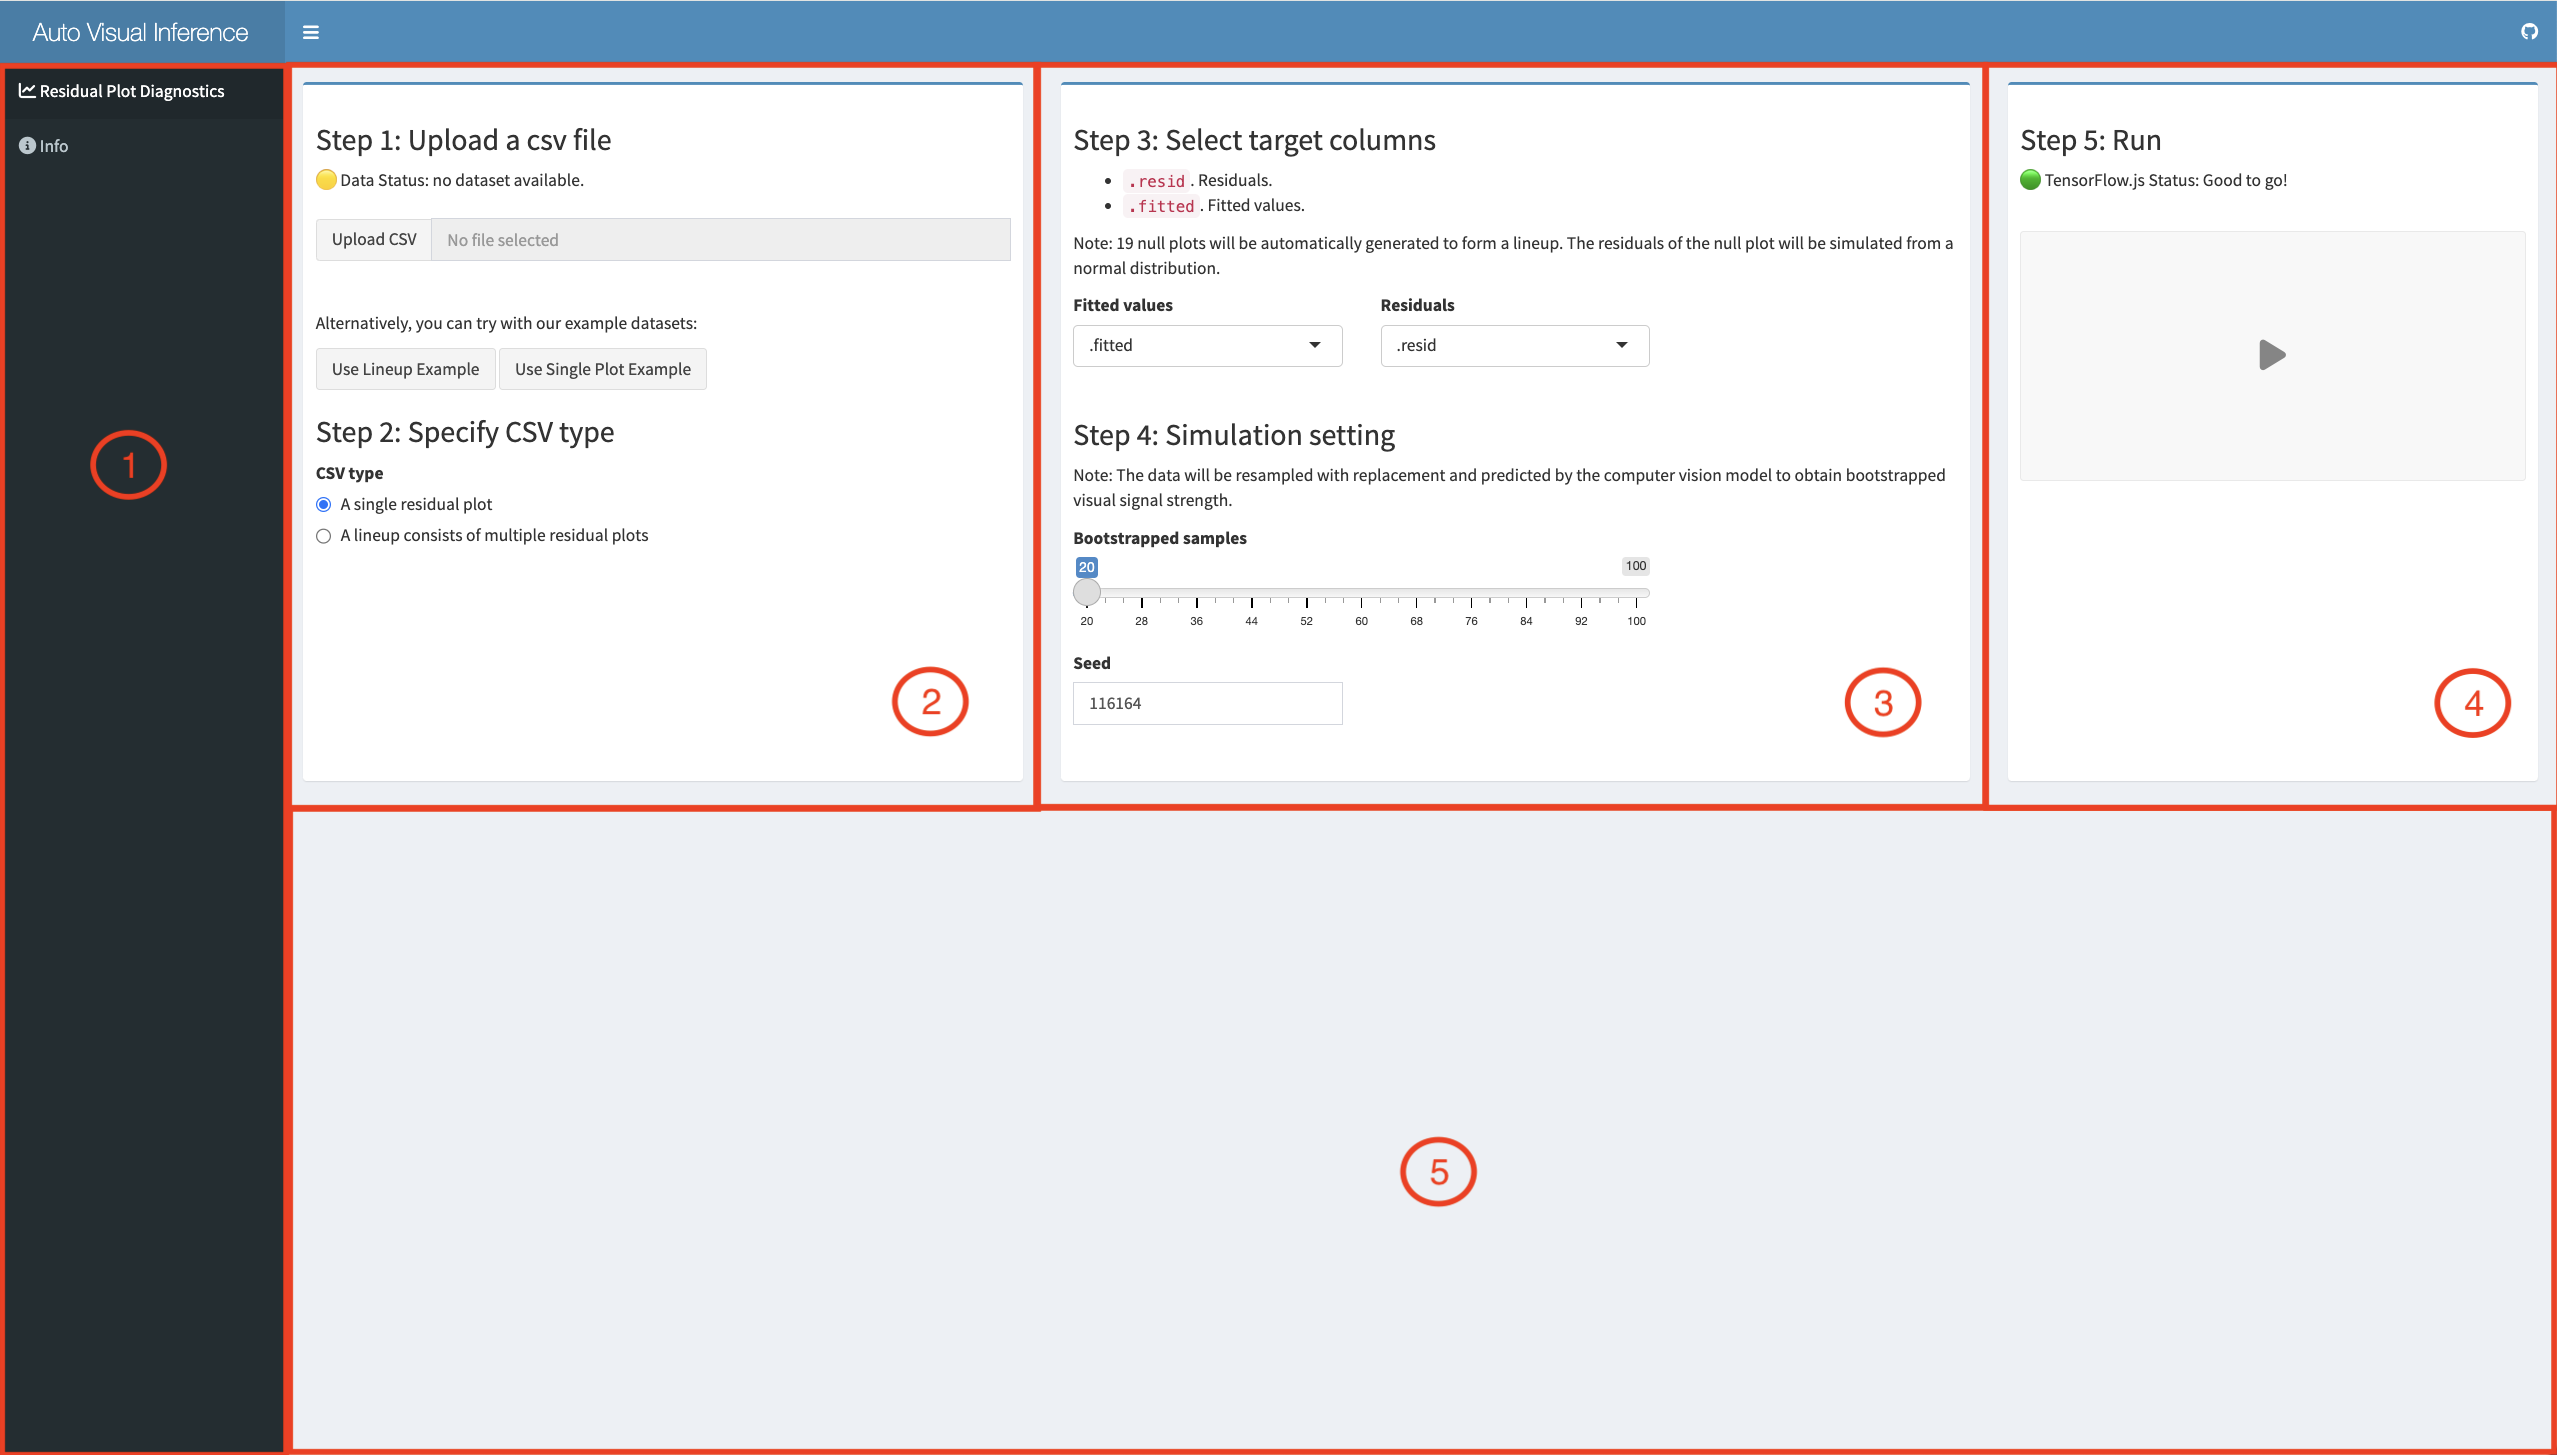
\includegraphics[width=1\textwidth,height=\textheight]{figures/autovi_web.png}

}

\caption{\label{fig-autovi-web}Overview of the \texttt{autovi.web}
graphical user interface (GUI). This default view may change based on
user interactions. Region 1 is the sidebar menu, containing the residual
assessment tab and the information tab. Region 2 is the data upload
panel, where users can provide a CSV file and specify the type of data
it contains. Region 3 includes dropdown menus for selecting the columns
to be analyzed, a slider to control the number of bootstrapping samples,
and a numeric input box for setting the simulation seed. Region 4
displays the initialization status and offers a button to start the
analysis. Region 5 is empty in the default view but will be populated
with results once the analysis is started.}

\end{figure}%

While the R package \texttt{autovi} aims to provide tools that can be
extended to broader visual inference applications, \texttt{autovi.web}
is only focus on providing a straightforward and clean user interface.
An overview of the graphical user interface of \texttt{autovi.web} is
provided in Figure~\ref{fig-autovi-web}. This is the default view of the
web application, and there are five regions that user can mainly
interact with. Region 1 of Figure~\ref{fig-autovi-web} is a sidebar menu
which can switch between the analysis page and the information page. The
analysis page is the focus of this section.

Region 2 of Figure~\ref{fig-autovi-web} is a panel for data uploading
and CSV type selection. Clicking the ``upload CSV'' button opens a
window where the user can select a file from their local system. The
data status displayed above the button provides information about the
number of rows and columns in the current dataset. Additionally, there
are two example datasets available beneath the ``upload CSV'' button:
one is a lineup example using a CSV file with three columns, and the
other is a single plot example using a CSV file with two columns. More
details about these example datasets are be discussed in
Section~\ref{sec-autovi-web-workflow}.

While the \texttt{autovi} package typically expects a fitted regression
model object provided by the user, this approach is impractical for a
web interface. Saving the R model object to the filesystem involves
extra steps and requires users to have specific knowledge, which does
not align with the goal of the web application. Moreover, the regression
model object may contain sensitive, non-shareable data, making it
unsuitable for uploading. Additionally, model objects are often
unnecessarily large, containing extra information not needed for
residual diagnostics. In contrast, a CSV file is easier to generate
using various software programs, not just R. CSV files are widely
accepted and can be easily viewed and modified using common desktop
applications like Excel. They are generally less sensitive than raw
data, as they exclude most information about the predictors.

The web application is designed to assess either a single residual plot
or a lineup of residual plots. Therefore, it accepts only two types of
CSV files: one with at least two columns representing the fitted values
and residuals of a single residual plot, and another with at least three
columns, where the additional column serves as the label or identifier
for a lineup of multiple residual plots. For a single residual plot, 19
null plots are generated by simulating normal random draws from a
distribution with the same variance as the original residual plot, and
comparisons are made with the original residual plot. For a lineup,
comparisons are made among the plots within the lineup. After uploading
the CSV file, the user must select the correct format to ensure the web
interface interprets the data correctly.

\begin{figure}

\centering{

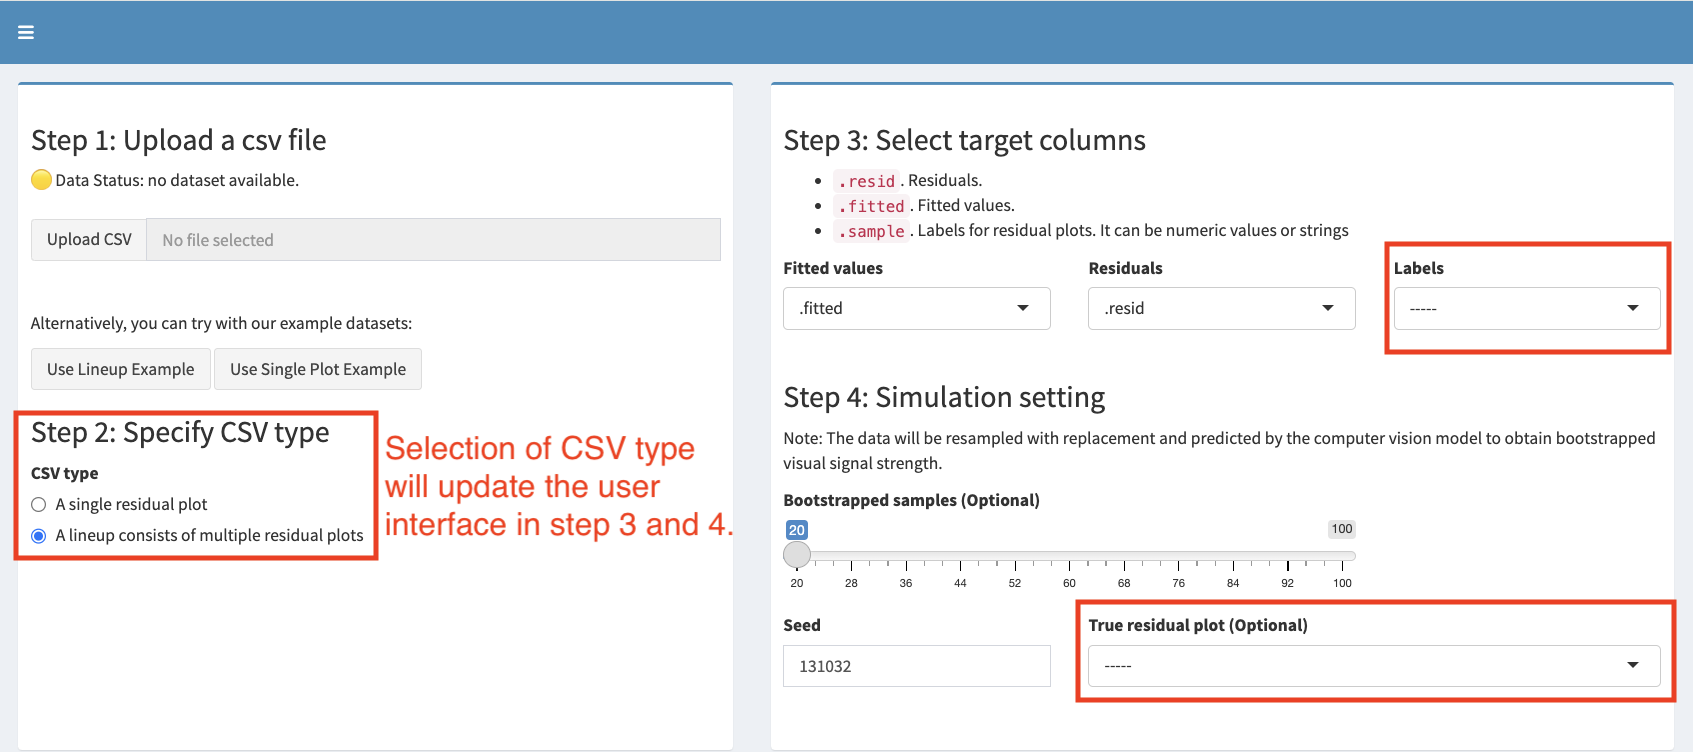
\includegraphics[width=1\textwidth,height=\textheight]{figures/autovi_web_type.png}

}

\caption{\label{fig-autovi-web-type}The panels for selecting target
columns and simulation settings are updated when a different CSV type is
selected in the left panel. Compared to Figure~\ref{fig-autovi-web},
where the CSV type is a single residual plot, choosing a CSV type that
includes a lineup of multiple residual plots adds a dropdown menu for
specifying a column for the residual plot identifier. Additionally, an
optional dropdown menu for specifying the true residual plot identifier
will appear under the simulation settings.}

\end{figure}%

Region 3 of Figure~\ref{fig-autovi-web} is a panel for column selection
and simulation settings. As shown in Figure~\ref{fig-autovi-web}, if the
CSV type is set to a single residual plot, there will be two dropdown
menus for specifying the columns for fitted values and residuals,
respectively. The default variable names for these columns are
\texttt{.fitted} and \texttt{.resid}. After uploading the CSV file, the
content of these dropdown menus will be updated to reflect the existing
columns in the dataset. As displayed in
Figure~\ref{fig-autovi-web-type}, for the CSV type that is a lineup of
multiple residual plots, an additional dropdown menu will appear for
specifying the column of residual plot labels. The default variable name
for this column is \texttt{.sample}. If this variable name does not
exist in the dataset, the dropdown menu will remain empty, allowing the
user to specify the correct column. The number of levels for each option
in this dropdown menu will be displayed to help avoid the selection of a
variable with too many levels, which could significantly slow down the
application due to extensive computation.

Under the simulation settings, there is a slider for specifying the
number of bootstrapped samples needed for the assessment. A higher value
on this slider will result in a more accurate bootstrap distribution
estimation, though it will require more computation time. The simulation
seed can be set in a numeric input box below the slider to control the
reproducibility of the assessment. By default, a random seed is set each
time the web page is refreshed. When the CSV type is a lineup of
multiple residual plots, an optional dropdown menu will appear next to
the simulation seed input box, allowing the user to specify an
identifier for the true residual plot. If no label is provided for the
true residual plot, the assessment will only estimate the VSS for each
residual plot in the lineup, without providing a \(p\)-value, as it
cannot be computed. Consequently, some result panels may be missing due
to insufficient information. This option is useful when the lineup
consists solely of null plots or if the user simply wants to obtain the
VSS for multiple residual plots.

Region 4 of Figure~\ref{fig-autovi-web} is the panel for triggering the
assessment. It contains a large play button to start the assessment.
Above the play button, a text message displays the status of
\texttt{TensorFlow.js}, allowing users to monitor whether the JavaScript
library and Keras model have been loaded correctly. The play button will
remain disabled until both the data status in Region 1 and the
\texttt{TensorFlow.js} status in Region 4 indicate that everything is
ready, with both showing a green status.

Once the play button is clicked, region 5 of Figure~\ref{fig-autovi-web}
will be populated with panels displaying the assessment results.
Generally, there will be four result panels, as shown in
Figure~\ref{fig-autovi-web-result} and
Figure~\ref{fig-autovi-web-result2}.

\begin{figure}

\centering{

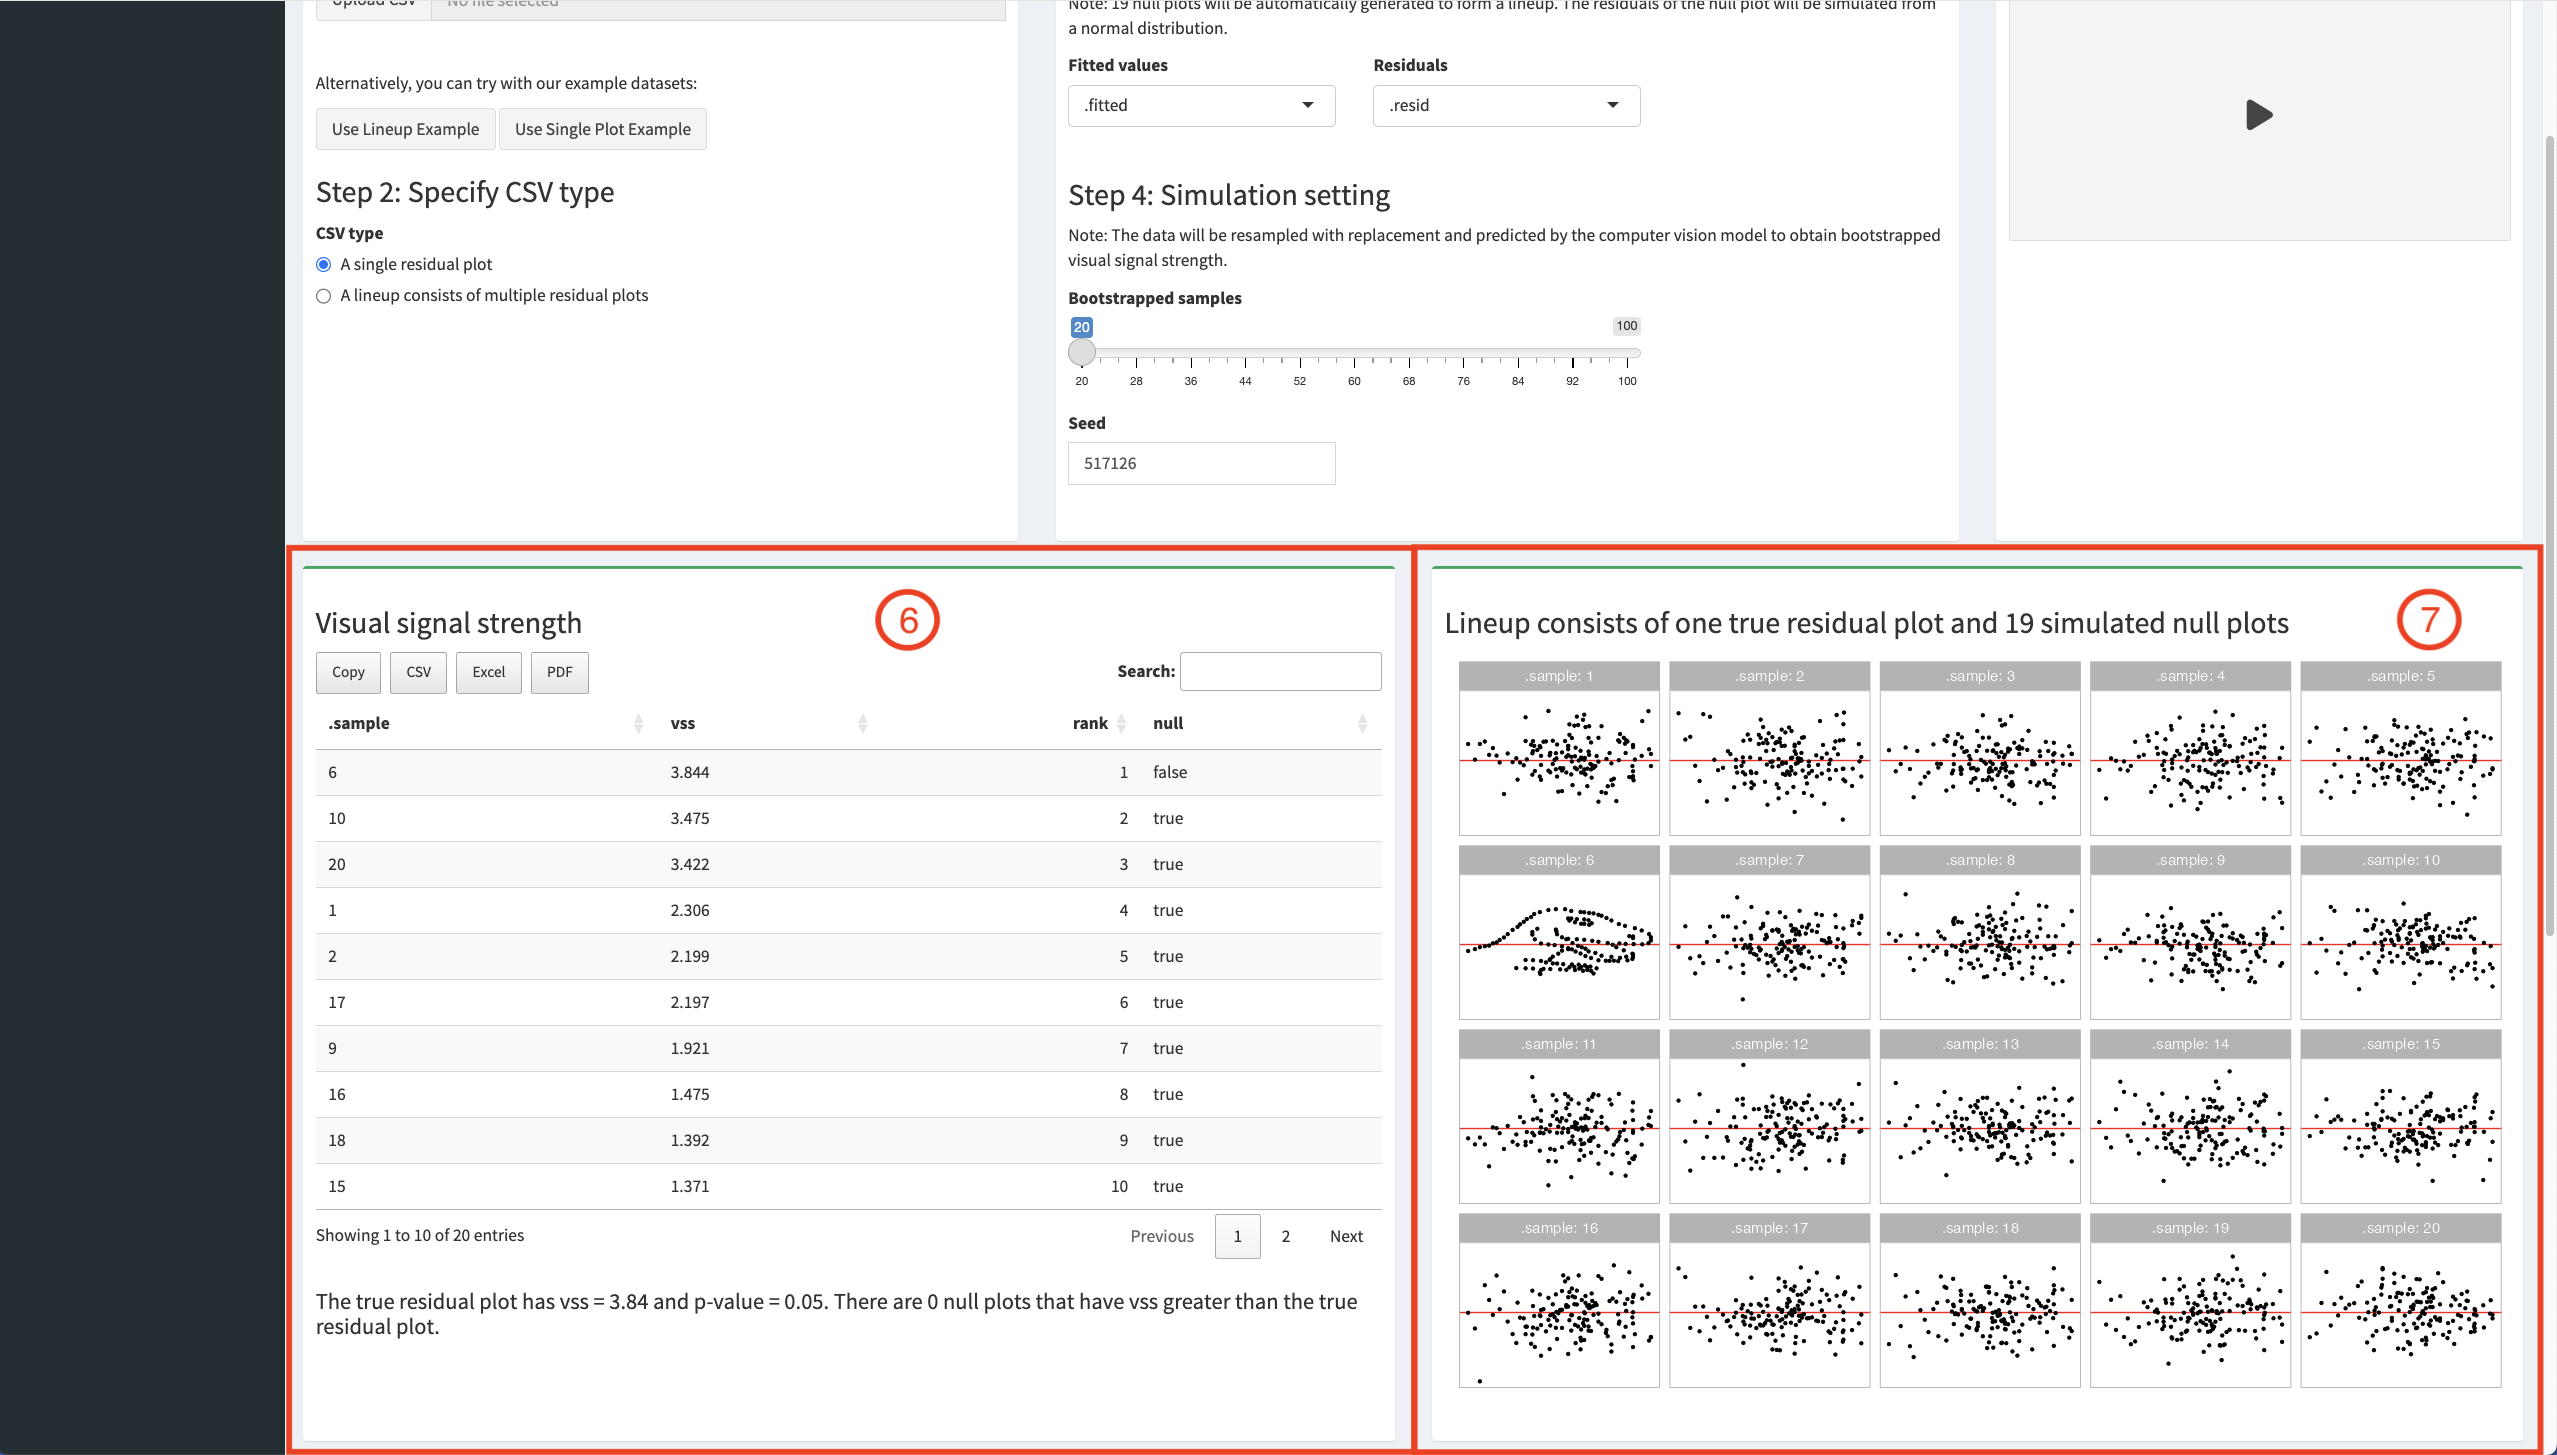
\includegraphics[width=1\textwidth,height=\textheight]{figures/autovi_web_result.png}

}

\caption{\label{fig-autovi-web-result}The first two panels of results
from the automated residual assessment are shown. The application
provides four results panels in total, and these screenshots display the
first two. In region 1, there is an interactive table detailing the VSS,
with a summary of the analysis provided in the paragraph below. Region 2
displays a lineup of residual plots.}

\end{figure}%

\begin{figure}

\centering{

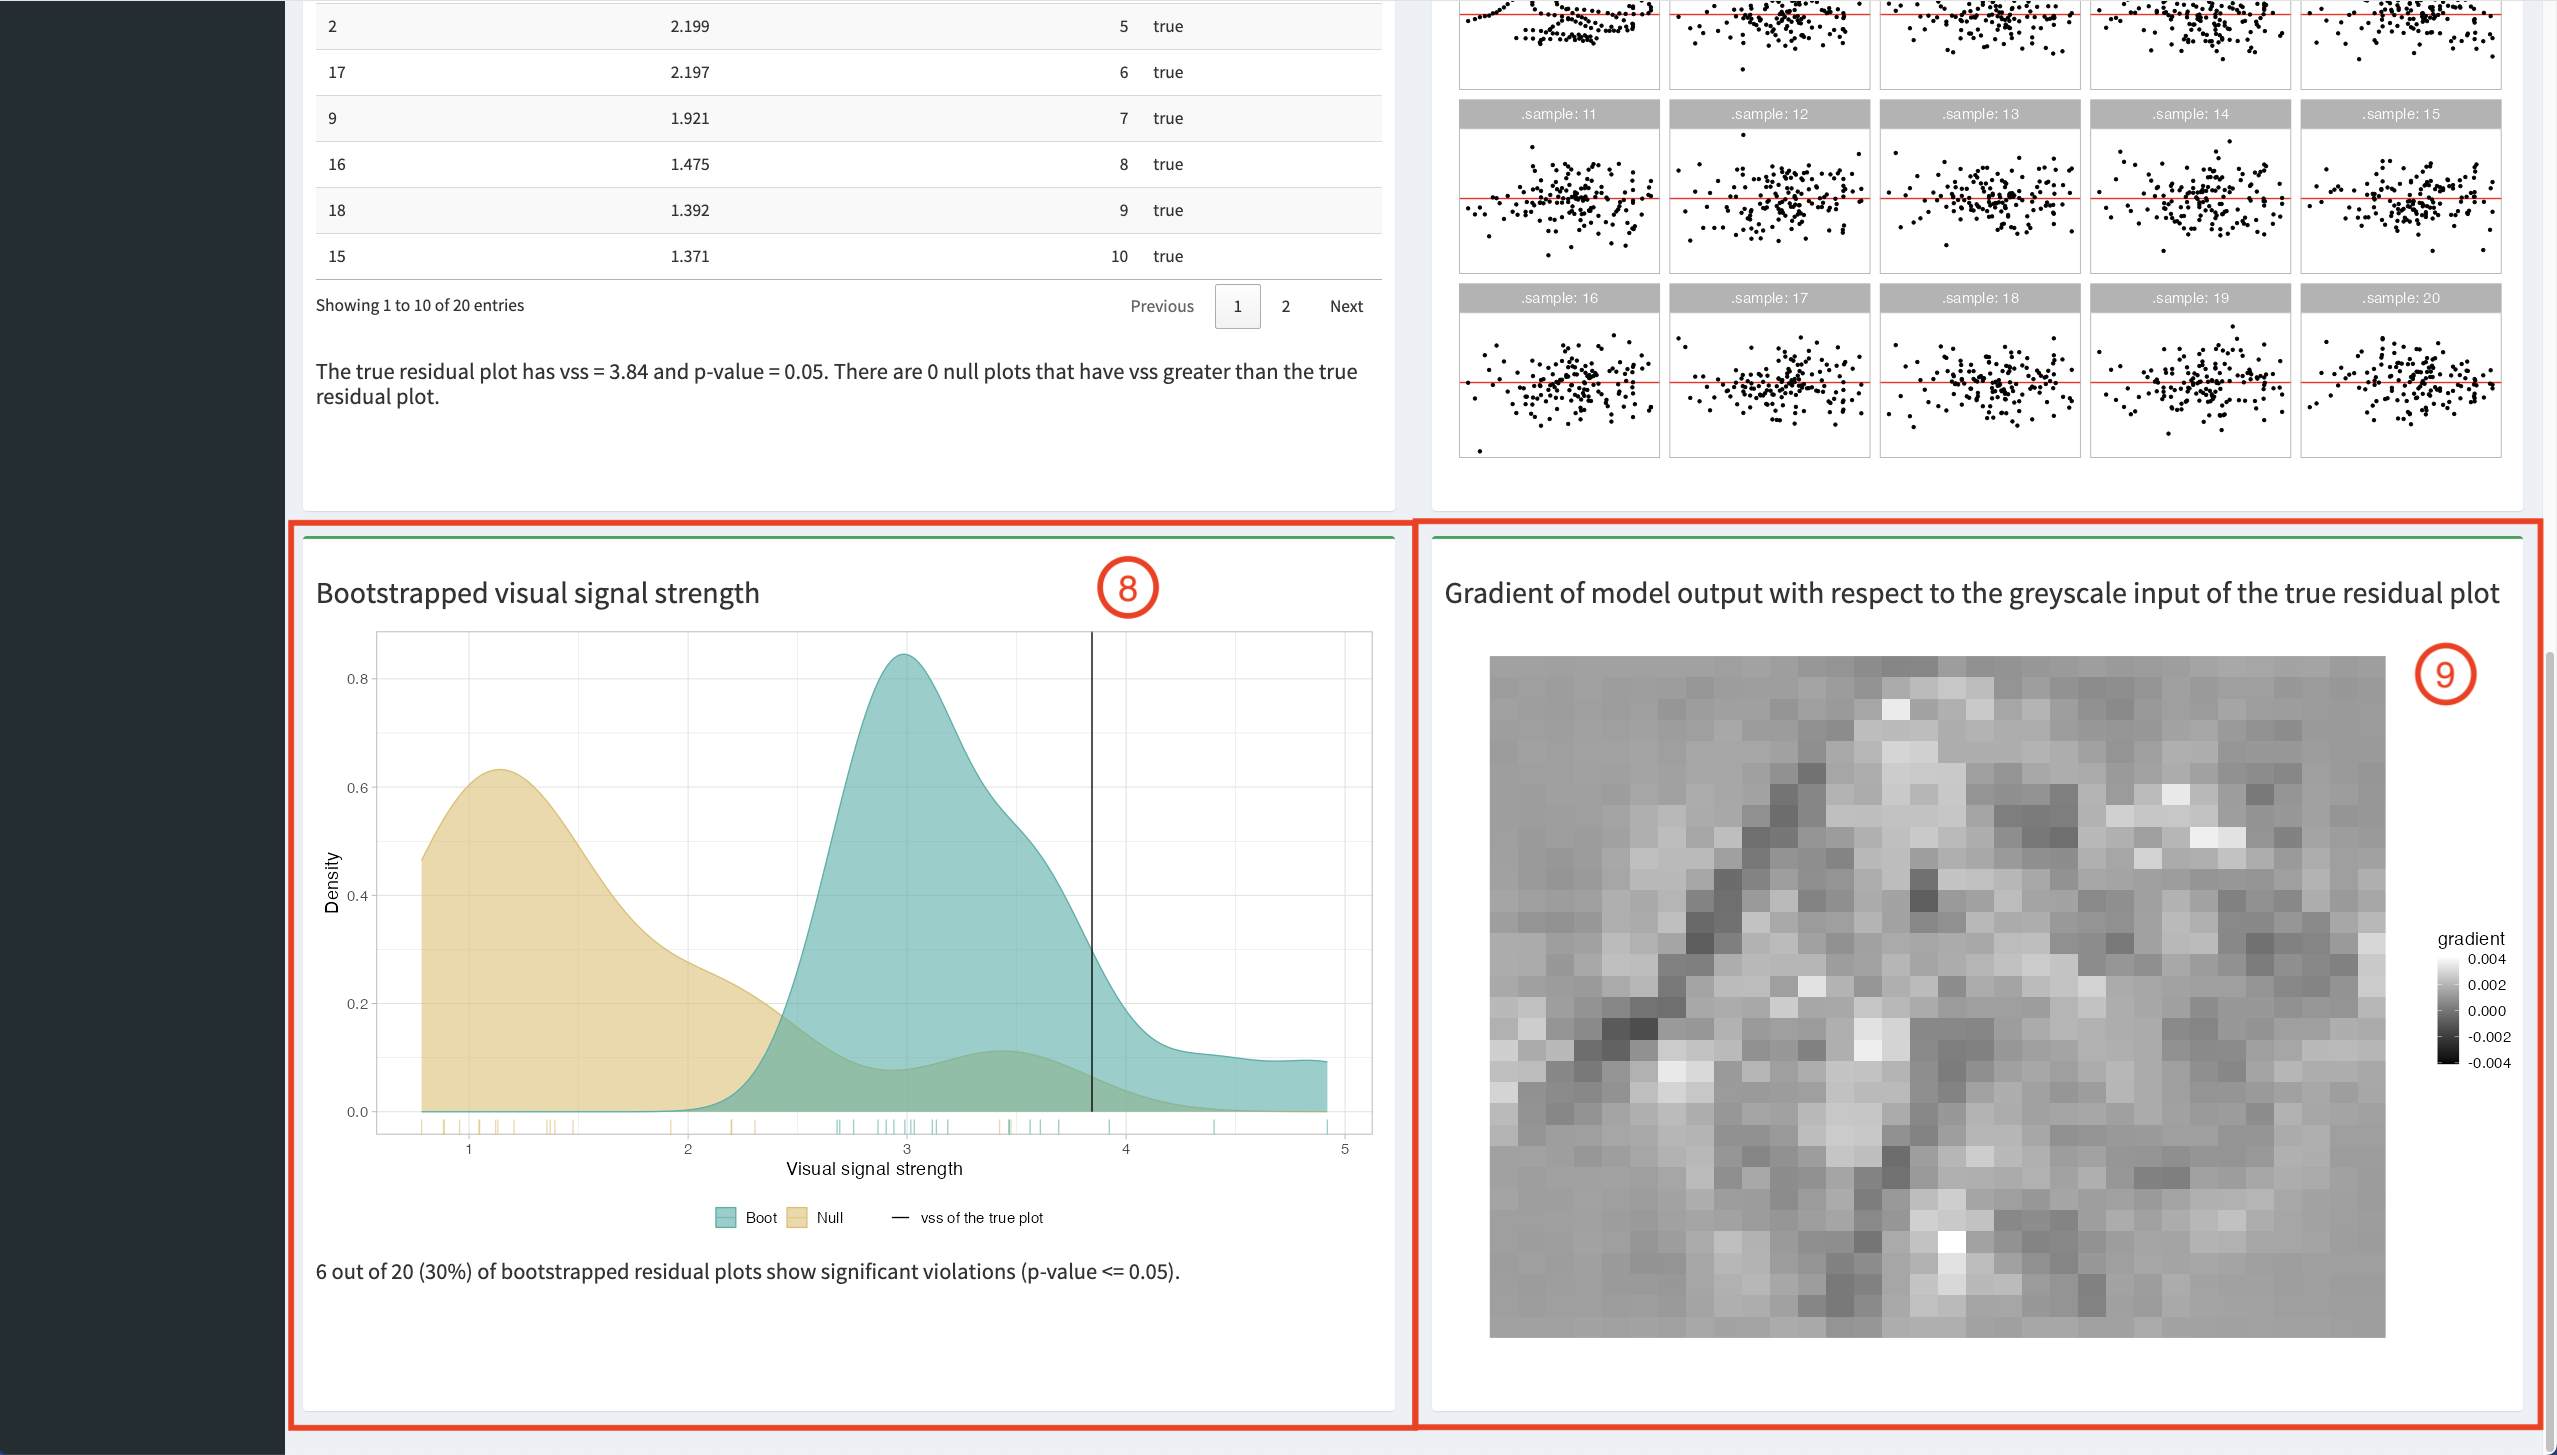
\includegraphics[width=1\textwidth,height=\textheight]{figures/autovi_web_result2.png}

}

\caption{\label{fig-autovi-web-result2}The last two panels of results
from the automated residual assessment are shown. The application
provides four results panels in total, and these screenshots display the
final two. Region 1 presents a density plot comparing the bootstrapped
VSS with the null VSS. Region 2 includes an attention map of the true
residual plot.}

\end{figure}%

\begin{figure}

\centering{

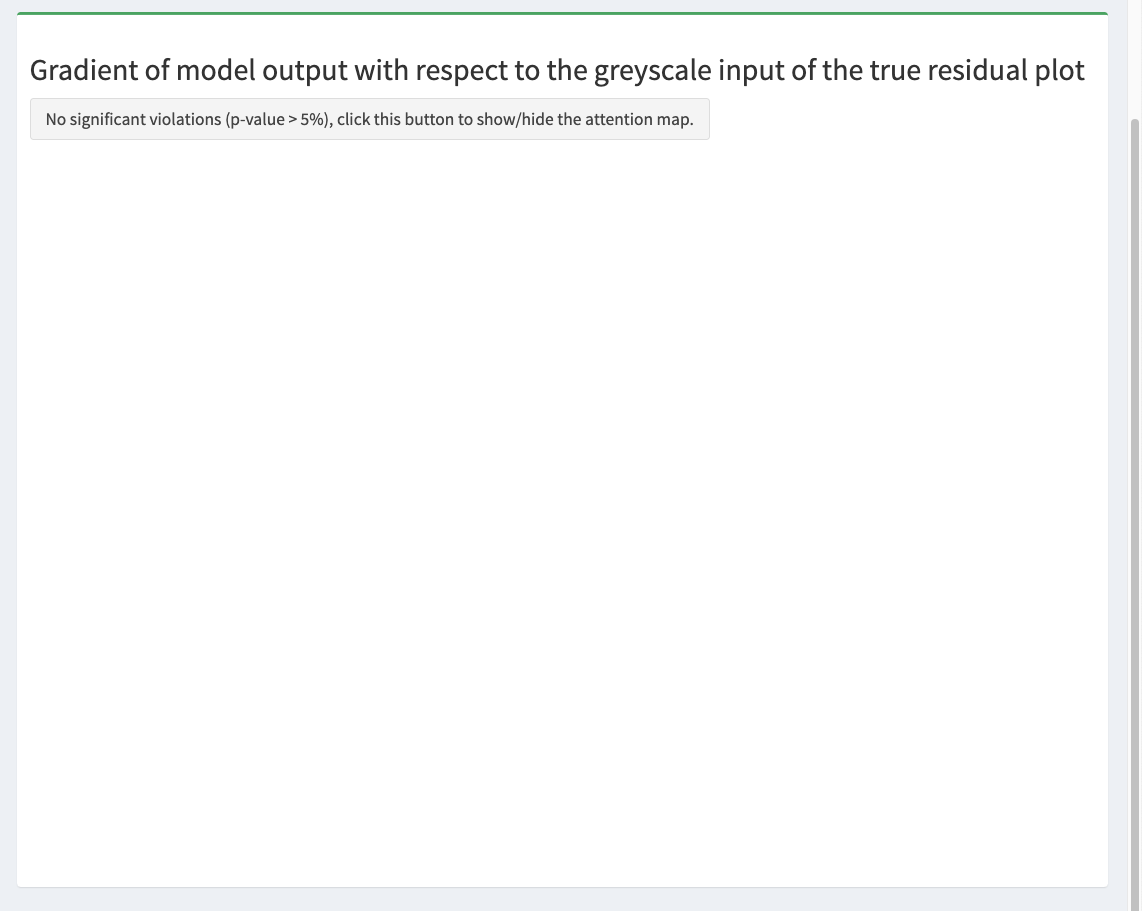
\includegraphics[width=0.5\textwidth,height=\textheight]{figures/autovi_web_gradient_hide.png}

}

\caption{\label{fig-autovi-web-gradient-hide}The attention map is hidden
if the assessment indicates a \(p\)-value greater than 0.05. A button is
available to toggle the display of the attention map.}

\end{figure}%

Region 6 of Figure~\ref{fig-autovi-web-result} contains an interactive
table created with the R package \texttt{DT} \citep{dt}, which provides
the VSS. This table includes four columns: \texttt{.sample},
\texttt{vss}, \texttt{rank}, and \texttt{null}. The \texttt{.sample}
column shows the residual plot labels. For a CSV type that is a lineup,
these labels are taken from an identifier column in the dataset
specified by the user. In the case of the CSV type is a single residual
plot, labels are automatically generated from 1 to 20, with the true
residual plot receiving a randomly assigned label. The \texttt{vss}
column displays the VSS for each residual plot, rounded to three decimal
places. The \texttt{rank} column indicates the ranking of each residual
plot based on VSS. The \texttt{null} column reveals whether the plot is
a null plot. For the CSV type that is a single residual plot, only the
true residual plot will have ``false'' in this column, while all other
plots will be marked ``true.'' For the CSV type that is a lineup, if the
true residual plot identifier has not been provided, this column will
show ``NA'' to represent missing values. If the identifier is provided
by user, the column behaves as if the CSV type is a single residual
plot.

The \texttt{DT} table provides several interactive features. Users can
download the table in four formats, including text, CSV, Excel, and PDF,
using the buttons located above the table. Additionally, the table is
searchable via the text input field also positioned above it. Below the
table, a text message displays the \(p\)-value of the assessment for the
true residual plot and summarizes the number of null plots with VSS
greater than that of the true residual plot. This helps the user
determine whether the true residual plot shows visual patterns that
suggest model violations.

Region 7 of Figure~\ref{fig-autovi-web-result} provides a lineup of
plots corresponding to each \texttt{.sample} value from the table in
Region 6. Due to space limitations, a maximum of 20 residual plots will
be displayed, ensuring that the true residual plot, if known, will be
included in the lineup. The plots are generated using \texttt{ggplot2},
the same as in \texttt{autovi}. Users can perform a visual test with
this lineup to check if the true residual plot is distinguishable from
the other plots, helping to determine the significance of model
violations.

Region 8 of Figure~\ref{fig-autovi-web-result2} displays the density
plot for bootstrapped VSS and null VSS. The densities are shown in
distinct colors that are friendly for colorblind users. A solid vertical
line marks the VSS of the true residual plot, while rug lines at the
bottom of the plot provide a clearer view of individual cases. Below the
plot, a text message indicates the number and percentage of bootstrapped
residual plots that would be rejected by the visual test when compared
to the null plots. Note that the bootstrapped residual plots in this
application are generated differently from \texttt{autovi}. Since we do
not have the R model object, we can not refit the regression model with
bootstrapped data. Instead, we bootstrap the residuals of the true
residual plot directly to obtain bootstrapped residual plots. As as
result, this panel will disappear when the true residual plot is
unknown.

Region 9 of Figure~\ref{fig-autovi-web-result2} displays an attention
map for the true residual plot, generated by computing the gradient of
the Keras model's output with respect to the greyscale input of the
plot. The attention map helps to understand how the Keras model predicts
VSS and which areas it is focusing on. We use a greyscale input because
it is easier to generate a clear attention map in this format, and it
usually conveys all the essential information, as most of the important
details of the plot are drawn in black. If the \(p\)-value of the true
residual plot is greater than 0.05, checking the attention map is not
necessary. However, to provide users with the option to review it if
they wish, a button will be available, as shown in
Figure~\ref{fig-autovi-web-gradient-hide}. This button allows users to
toggle the display of the attention map.

\subsection{Workflow}\label{sec-autovi-web-workflow}

The workflow of \texttt{autovi.web} is designed to be straightforward,
with numbered steps displayed in each panel shown in
Figure~\ref{fig-autovi-web}. There are two example datasets provided by
the web application, as mentioned in
Section~\ref{sec-autovi-web-design}. The single residual plot example
uses the \texttt{dino} dataset from the R package \texttt{datasauRus}
\citep{datasaurus}. The lineup example uses residuals from a simulated
regression model that has a non-linearity issue. We will walk through
the lineup example to further demonstrate the workflow of the web
application.

As shown in Figure~\ref{fig-autovi-web-workflow-example1}, to use the
lineup example data, click the ``Use Lineup Example'' button. The data
status will then update to show the number of rows and columns in the
dataset, and the CSV type will automatically be selected to the correct
option. Since the example dataset follows the variable naming
conventions assumed by the web application, the columns for fitted
values, residuals, and labels of residual plots are set automatically
(Figure~\ref{fig-autovi-web-workflow-example2}). If the user is working
with a custom dataset, these options must be set accordingly. Regardless
of the dataset, the user must manually select the label for the true
residual plot, as the web application allows assessments without this
label. The next step is to click the play button to start the
assessment.

Results are provided in multiple panels as displayed in
Figure~\ref{fig-autovi-web-workflow-example3},
Figure~\ref{fig-autovi-web-workflow-example4},
Figure~\ref{fig-autovi-web-workflow-example5} and
Figure~\ref{fig-autovi-web-workflow-example6}. In
Figure~\ref{fig-autovi-web-workflow-example3}, the first row of the
table is the most crucial to check, as it provides the VSS and the rank
of the true residual plot among the other plots. The summary text
beneath the table provides the \(p\)-value, which can be used for quick
decision-making. In Figure~\ref{fig-autovi-web-workflow-example4}, the
lineup is for manual inspection, and the user should see if the true
residual plot is visually distinguishable from the other plots, to
confirm if the model violation is serious. The density plot in
Figure~\ref{fig-autovi-web-workflow-example5} offers a more robust
result, allowing the user to compare the distribution of bootstrapped
VSS with the distribution of null VSS. Finally, the grayscale attention
map shown in Figure~\ref{fig-autovi-web-workflow-example6} can be used
to check if the target visual features, like the non-linearity present
in the lineup example, are captured by the computer vision model,
ensuring the quality of the assessment.

\begin{figure}

\centering{

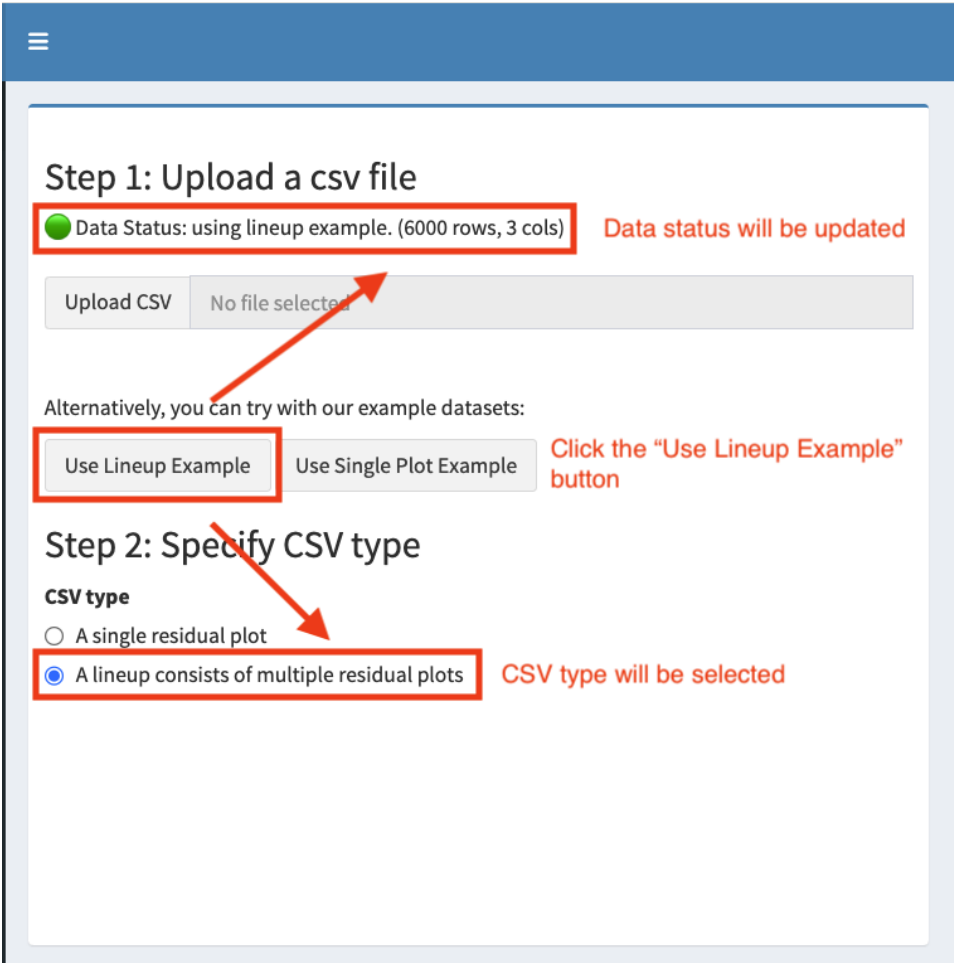
\includegraphics[width=0.8\textwidth,height=\textheight]{autovi_paper_files/figure-pdf/fig-autovi-web-workflow-example1-1.png}

}

\caption{\label{fig-autovi-web-workflow-example1}To begin the workflow
for \texttt{autovi} using the lineup example dataset, the user clicks
the ``Use Lineup Example'' button to load the example dataset, during
which the data status and CSV type will be automatically updated.}

\end{figure}%

\begin{figure}

\centering{

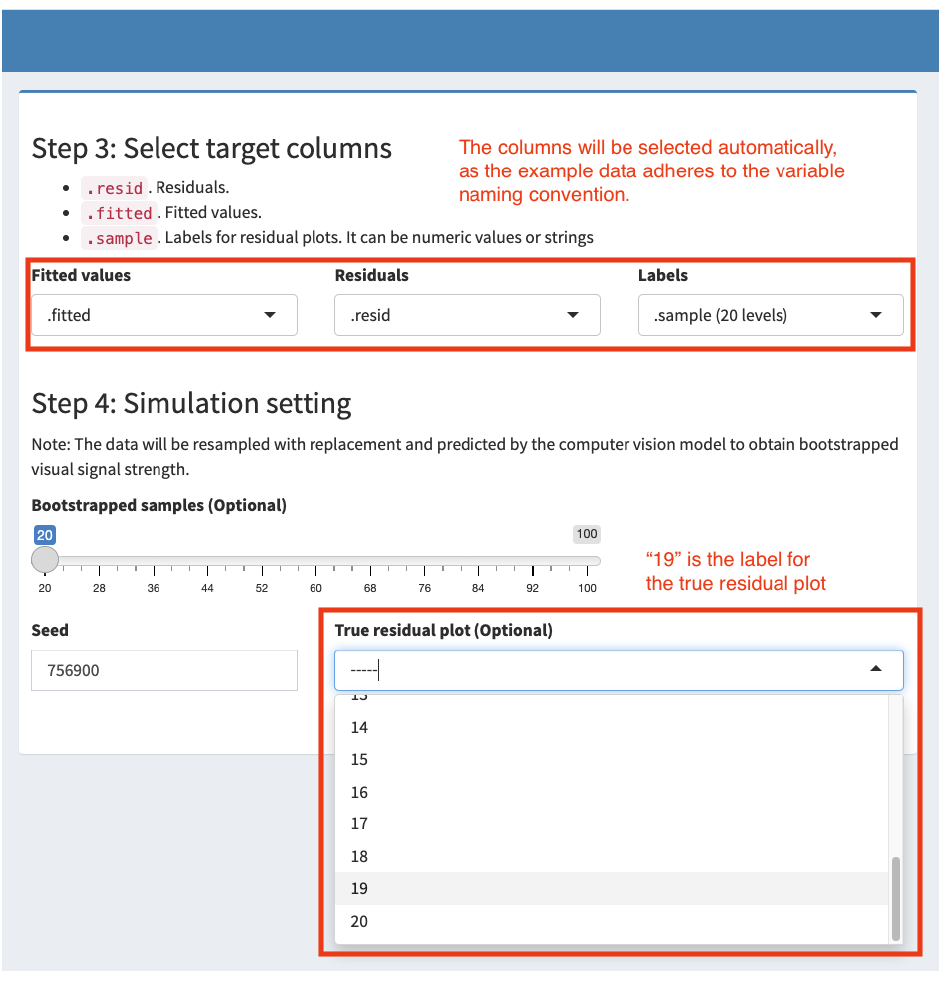
\includegraphics[width=0.8\textwidth,height=\textheight]{autovi_paper_files/figure-pdf/fig-autovi-web-workflow-example2-1.png}

}

\caption{\label{fig-autovi-web-workflow-example2}After clicking the
button in Figure~\ref{fig-autovi-web-workflow-example1}, the target
columns are selected automatically, though the user must manually select
the label for the true residual plot, as the web application permits
assessment without this label.}

\end{figure}%

\begin{figure}

\centering{

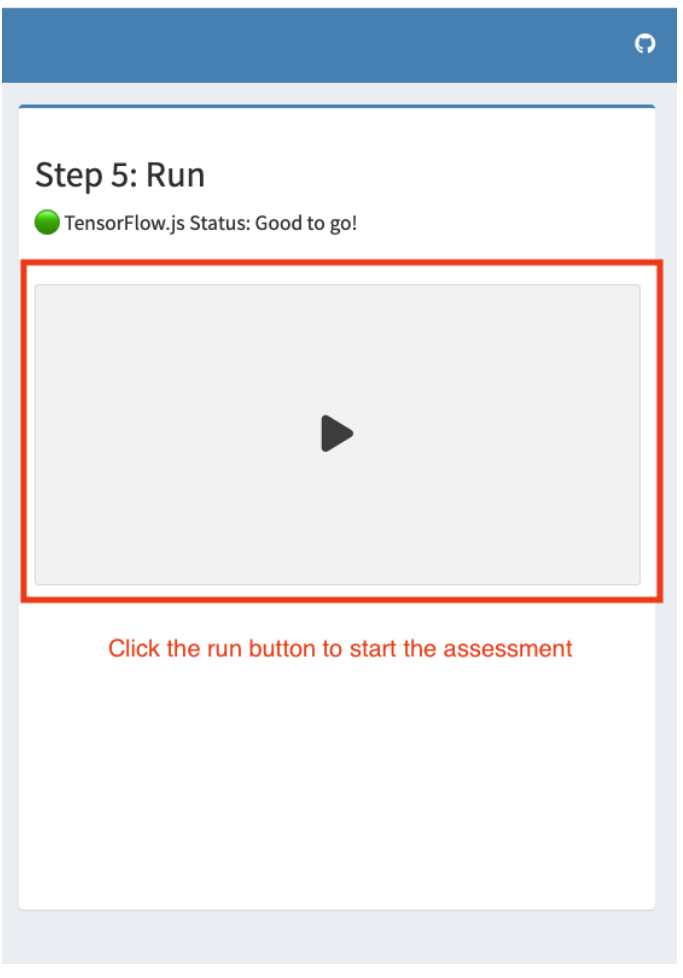
\includegraphics[width=0.55\textwidth,height=\textheight]{autovi_paper_files/figure-pdf/fig-autovi-web-workflow-example3-1.png}

}

\caption{\label{fig-autovi-web-workflow-example3}After finishing the
required steps in Figure~\ref{fig-autovi-web-workflow-example1} and
Figure~\ref{fig-autovi-web-workflow-example2}, the user initiates the
assessment of the lineup example data by clicking the run button.}

\end{figure}%

\begin{figure}

\centering{

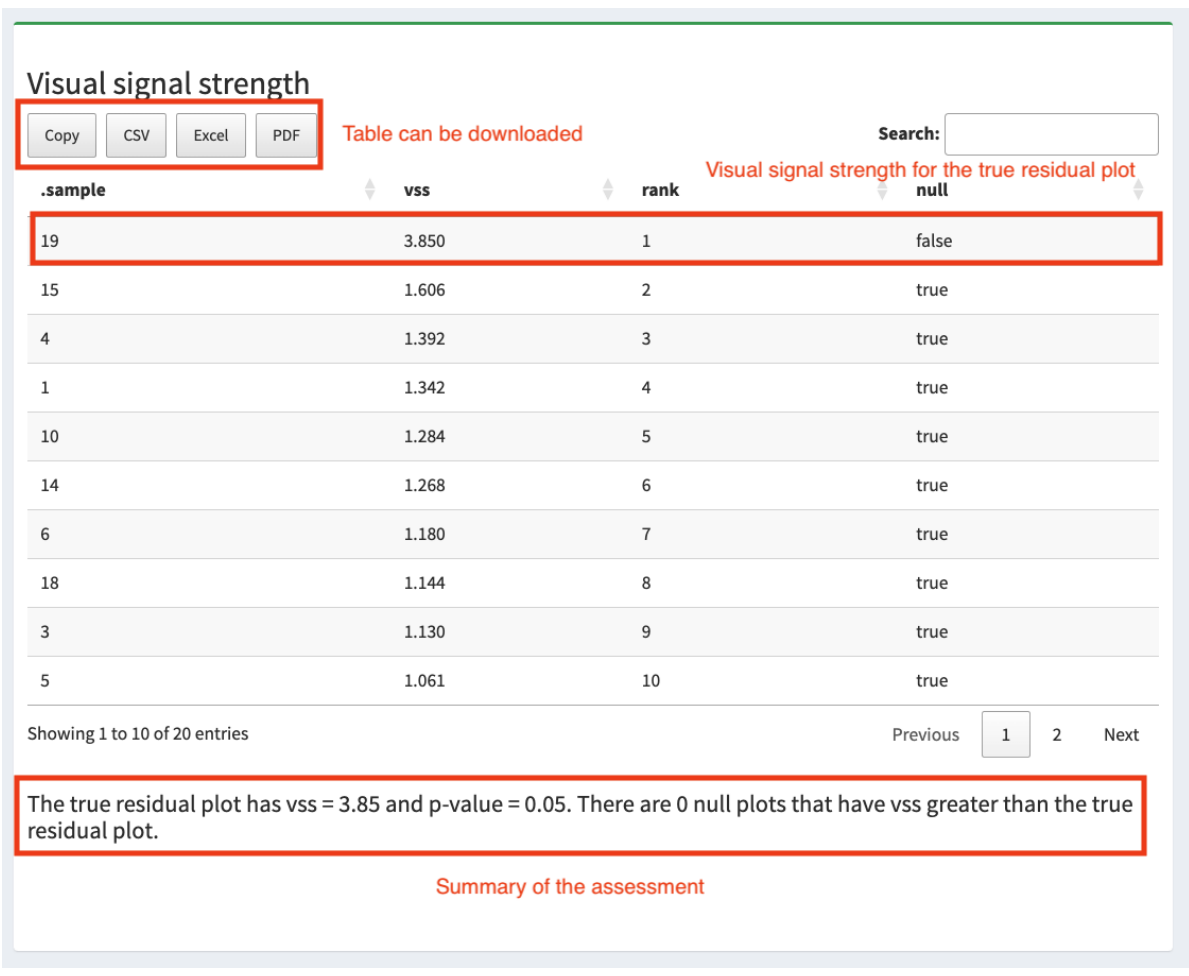
\includegraphics[width=1\textwidth,height=\textheight]{autovi_paper_files/figure-pdf/fig-autovi-web-workflow-example4-1.png}

}

\caption{\label{fig-autovi-web-workflow-example4}The VSS of the true
residual plot is displayed in the first row of the table, with a summary
text beneath the table providing the \(p\)-value to aid in
decision-making.}

\end{figure}%

\begin{figure}

\centering{

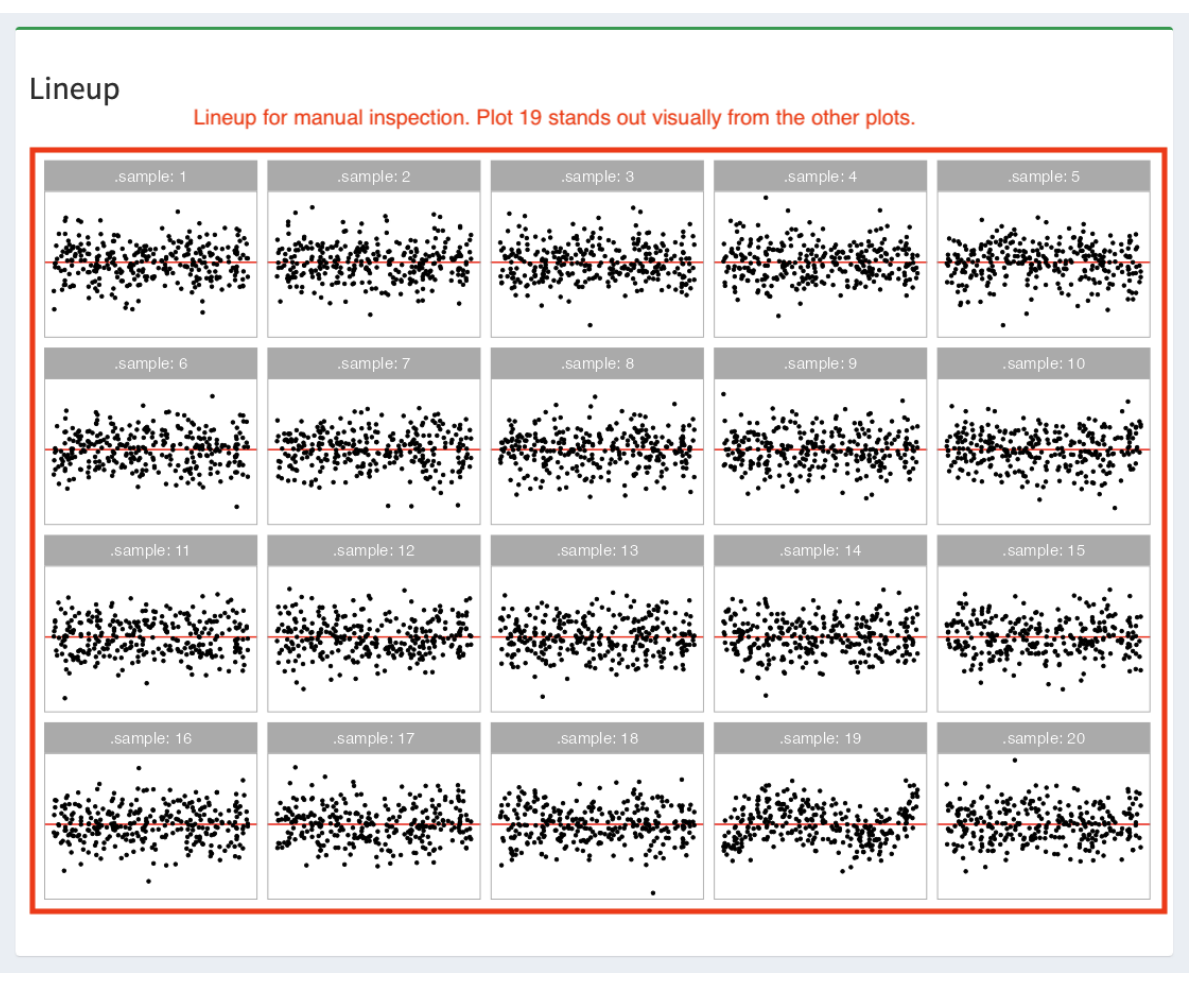
\includegraphics[width=1\textwidth,height=\textheight]{autovi_paper_files/figure-pdf/fig-autovi-web-workflow-example5-1.png}

}

\caption{\label{fig-autovi-web-workflow-example5}A lineup of residual
plots allows for manual inspection.}

\end{figure}%

\begin{figure}

\centering{

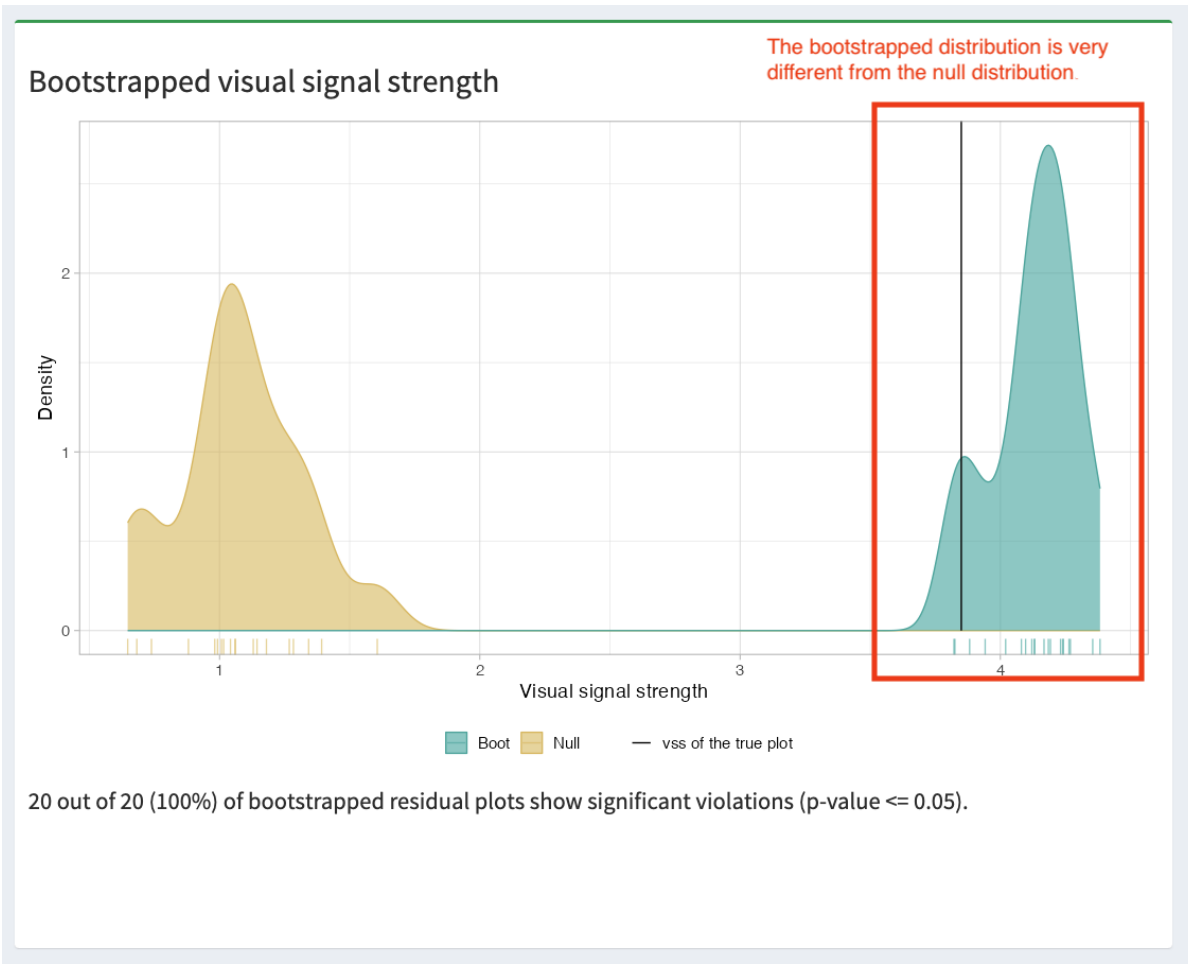
\includegraphics[width=1\textwidth,height=\textheight]{autovi_paper_files/figure-pdf/fig-autovi-web-workflow-example6-1.png}

}

\caption{\label{fig-autovi-web-workflow-example6}The density plot helps
verify if the bootstrapped distribution differs from the null
distribution.}

\end{figure}%

\begin{figure}

\centering{

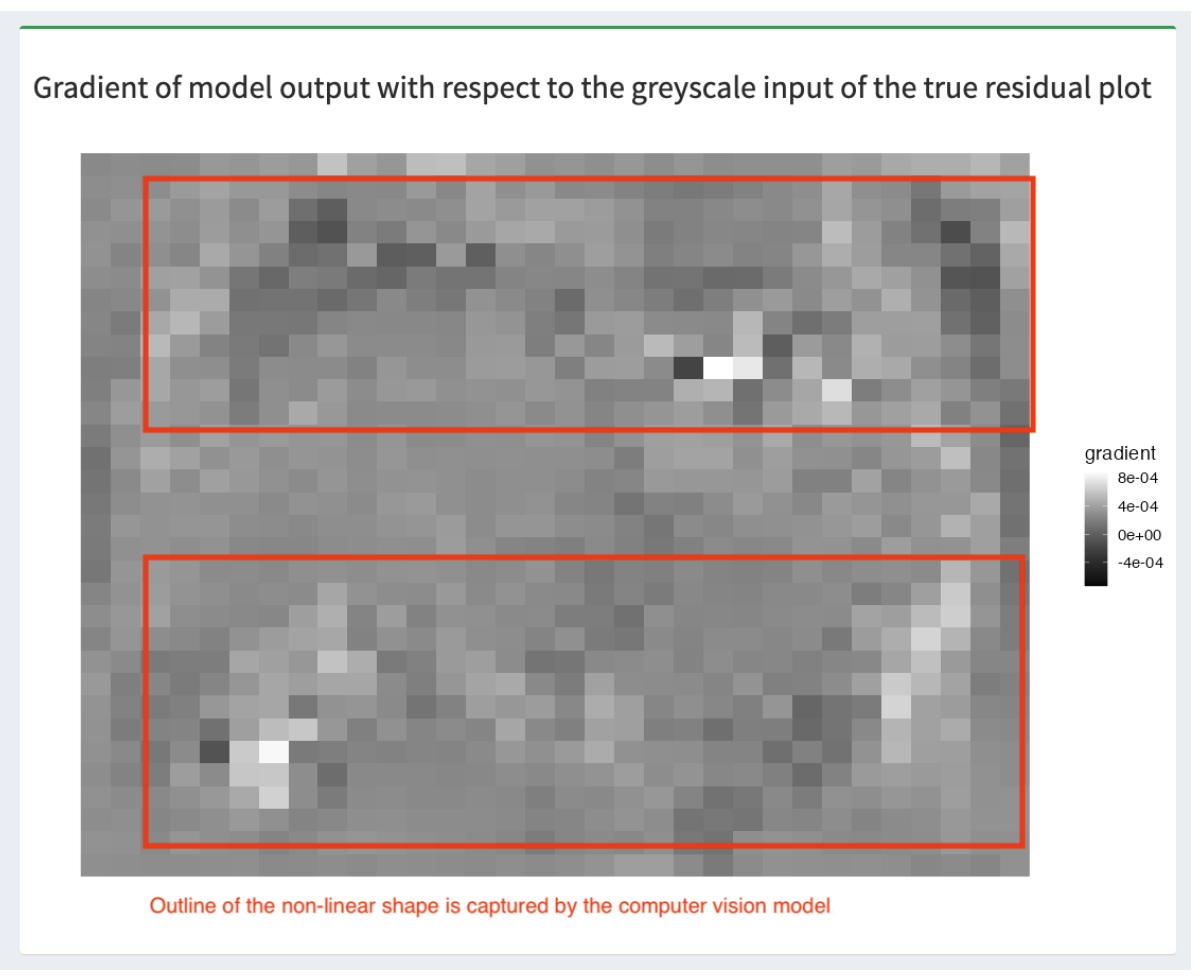
\includegraphics[width=1\textwidth,height=\textheight]{autovi_paper_files/figure-pdf/fig-autovi-web-workflow-example7-1.png}

}

\caption{\label{fig-autovi-web-workflow-example7}The attention map
offers insights into whether the computer vision model has captured the
intended visual features of the true residual plot.}

\end{figure}%

\section{Conclusions}\label{sec-autovi-conclusion}

This paper presents new regression diagnostics software, the R package
\texttt{autovi} and its accompanying web interface package,
\texttt{autovi.web}. It addresses a critical gap in the current
landscape of statistical software. While regression tools are widely
available, effective and efficient diagnostic methods have lagged
behind, particularly in the field of residual plot interpretation.

The \texttt{autovi} R package, introduced in this paper, automates the
assessment of residual plots by incorporating a computer vision model,
eliminating the need for time-consuming and potentially inconsistent
human interpretation. This automation improves the efficiency of the
diagnostic process and promotes consistency in model evaluation across
different users and studies.

The development of the accompanying Shiny app, \texttt{autovi.web},
expands access to these advanced diagnostic tools, by providing a
user-friendly interface. It makes automated residual plot assessment
accessible to a broader audience, including those who may not have
extensive programming experience. This web-based solution effectively
addresses the potential barriers to adoption, such as complex
dependencies and installation requirements, that are often associated
with advanced statistical software.

The combination of \texttt{autovi} and \texttt{autovi.web} offers a
comprehensive solution to the challenges of residual plot interpretation
in regression analysis. These tools have the potential to significantly
improve the quality and consistency of model diagnostics across various
fields, from academic research to industry applications. By automating a
critical aspect of model evaluation, they allow researchers and analysts
to focus more on interpreting results and refining models, rather than
grappling with the intricacies of plot assessment.

The framework established by \texttt{autovi} and \texttt{autovi.web}
opens up exciting possibilities for further research and development.
Future work could explore the extension of these automated assessment
techniques to other types of diagnostic plots and statistical models,
potentially revolutionizing how we approach statistical inference using
visual displays more broadly.

\section{Availability}\label{availability}

The web interface is housed at \url{autoviweb.netlify.app}.

The the current version of \texttt{autovi} can be installed from CRAN,
and source code for both packages are available at
\url{https://github.com/TengMCing/}.


  \bibliography{bibliography.bib}



\end{document}
